\PassOptionsToPackage{unicode=true}{hyperref} % options for packages loaded elsewhere
\PassOptionsToPackage{hyphens}{url}
%
\documentclass[]{book}
\usepackage{lmodern}
\usepackage{amssymb,amsmath}
\usepackage{ifxetex,ifluatex}
\usepackage{fixltx2e} % provides \textsubscript
\ifnum 0\ifxetex 1\fi\ifluatex 1\fi=0 % if pdftex
  \usepackage[T1]{fontenc}
  \usepackage[utf8]{inputenc}
  \usepackage{textcomp} % provides euro and other symbols
\else % if luatex or xelatex
  \usepackage{unicode-math}
  \defaultfontfeatures{Ligatures=TeX,Scale=MatchLowercase}
\fi
% use upquote if available, for straight quotes in verbatim environments
\IfFileExists{upquote.sty}{\usepackage{upquote}}{}
% use microtype if available
\IfFileExists{microtype.sty}{%
\usepackage[]{microtype}
\UseMicrotypeSet[protrusion]{basicmath} % disable protrusion for tt fonts
}{}
\IfFileExists{parskip.sty}{%
\usepackage{parskip}
}{% else
\setlength{\parindent}{0pt}
\setlength{\parskip}{6pt plus 2pt minus 1pt}
}
\usepackage{hyperref}
\hypersetup{
            pdftitle={CM 2110 Calculus and Statistical Distributions},
            pdfauthor={Dr.~Priyanga D. Talagala},
            pdfborder={0 0 0},
            breaklinks=true}
\urlstyle{same}  % don't use monospace font for urls
\usepackage{longtable,booktabs}
% Fix footnotes in tables (requires footnote package)
\IfFileExists{footnote.sty}{\usepackage{footnote}\makesavenoteenv{longtable}}{}
\usepackage{graphicx,grffile}
\makeatletter
\def\maxwidth{\ifdim\Gin@nat@width>\linewidth\linewidth\else\Gin@nat@width\fi}
\def\maxheight{\ifdim\Gin@nat@height>\textheight\textheight\else\Gin@nat@height\fi}
\makeatother
% Scale images if necessary, so that they will not overflow the page
% margins by default, and it is still possible to overwrite the defaults
% using explicit options in \includegraphics[width, height, ...]{}
\setkeys{Gin}{width=\maxwidth,height=\maxheight,keepaspectratio}
\setlength{\emergencystretch}{3em}  % prevent overfull lines
\providecommand{\tightlist}{%
  \setlength{\itemsep}{0pt}\setlength{\parskip}{0pt}}
\setcounter{secnumdepth}{5}
% Redefines (sub)paragraphs to behave more like sections
\ifx\paragraph\undefined\else
\let\oldparagraph\paragraph
\renewcommand{\paragraph}[1]{\oldparagraph{#1}\mbox{}}
\fi
\ifx\subparagraph\undefined\else
\let\oldsubparagraph\subparagraph
\renewcommand{\subparagraph}[1]{\oldsubparagraph{#1}\mbox{}}
\fi

% set default figure placement to htbp
\makeatletter
\def\fps@figure{htbp}
\makeatother

\usepackage{booktabs}
\usepackage{amsthm}
\makeatletter
\def\thm@space@setup{%
  \thm@preskip=8pt plus 2pt minus 4pt
  \thm@postskip=\thm@preskip
}
\makeatother
\usepackage{fancyhdr}
\pagestyle{fancy}
\fancyfoot[CO,CE]{Prepared by Dr. Priyanga D. Talagala}
\fancyfoot[LE,RO]{\thepage}
\usepackage{wrapfig}
\usepackage{floatrow}
\floatplacement{figure}{H}
\floatplacement{table}{H}
\makeatletter\renewcommand*{\fps@figure}{H}\makeatother
\usepackage{mathtools}
\usepackage{pdflscape}
\newcommand{\blandscape}{\begin{landscape}}
\newcommand{\elandscape}{\end{landscape}}
\usepackage[]{natbib}
\bibliographystyle{apalike}

\title{CM 2110 Calculus and Statistical Distributions}
\author{Dr.~Priyanga D. Talagala}
\date{2020-08-21}

\begin{document}
\maketitle

{
\setcounter{tocdepth}{1}
\tableofcontents
}
\hypertarget{course-syllabus}{%
\chapter*{Course Syllabus}\label{course-syllabus}}
\addcontentsline{toc}{chapter}{Course Syllabus}

\hypertarget{pre-requisites}{%
\section*{Pre-requisites}\label{pre-requisites}}
\addcontentsline{toc}{section}{Pre-requisites}

CM 1110

\textbf{Remark:}

\emph{This course module contains two main sections: (1) mathematics and (2) statistics. This syllabus is designed for the statistics section. Lectures for mathematics section and statistics section are conducted by two lecturers as two separate sub modules (1.5 hour lectures/Week). End Semester Examination is conducted as a single examination.}

\hypertarget{learning-outcomes}{%
\section*{Learning Outcomes}\label{learning-outcomes}}
\addcontentsline{toc}{section}{Learning Outcomes}

On successful completion of this module, students will be able to plan more carefully the design of experiment in advance which provide evidence for or against theories of cause and effect and make inferences about population characteristics based on sample information and thereby solve data analysis problems in different application domains. (R(\url{https://cran.r-project.org/}) and RStudio are also freely available to install on your own computer). Get the Open Source Edition of RStudio Desktop. RStudio allows you to run R in a more user-friendly environment.

\hypertarget{outline-syllabus}{%
\section*{Outline Syllabus}\label{outline-syllabus}}
\addcontentsline{toc}{section}{Outline Syllabus}

\begin{itemize}
\tightlist
\item
  Functions of Several Variables
\item
  Linear Algebra
\item
  Coordinate Systems \& Vectors
\item
  Differential Equations
\item
  \textbf{Statistical Distributions}
\item
  \textbf{Estimation}
\item
  \textbf{Hypothesis Testing}
\item
  \textbf{Design of Experiments}
\end{itemize}

\hypertarget{method-of-assessment}{%
\section*{Method of Assessment}\label{method-of-assessment}}
\addcontentsline{toc}{section}{Method of Assessment}

\begin{itemize}
\tightlist
\item
  Mid-semester examination
\item
  End-semester examination
\end{itemize}

\hypertarget{recommended-texts}{%
\section*{Recommended Texts}\label{recommended-texts}}
\addcontentsline{toc}{section}{Recommended Texts}

\begin{itemize}
\tightlist
\item
  Casella, G., \& Berger, R. L. (2002). Statistical inference (Vol. 2, pp.~337-472). Pacific Grove, CA: Duxbury.
\item
  Mood, A.M., Graybill, F.A. and Boes, D.C. (2007): Introduction to the Theory of Statistics, 3rd Edn.
  (Reprint). Tata McGraw-Hill Pub. Co.~Ltd.~
\item
  Montgomery, D. C. (2017). Design and analysis of experiments. John wiley \& sons.
\end{itemize}

\hypertarget{lecturer}{%
\section*{Lecturer}\label{lecturer}}
\addcontentsline{toc}{section}{Lecturer}

Dr.~Priyanga D. Talagala

\hypertarget{schedule}{%
\section*{Schedule}\label{schedule}}
\addcontentsline{toc}{section}{Schedule}

Lectures:

\begin{itemize}
\tightlist
\item
  Friday {[}9.15 am - 10.45 am{]}
\end{itemize}

Tutorial:

\begin{itemize}
\tightlist
\item
  Friday {[}11.00 am - 12.30 pm{]}
\end{itemize}

Consultation time:

\begin{itemize}
\tightlist
\item
  Friday {[}8.15 am to 9.00 am{]}
\end{itemize}

\hypertarget{statistical-distributions}{%
\chapter{Statistical Distributions}\label{statistical-distributions}}

\pagenumbering{arabic}

\hypertarget{recap-cm-1110-probability}{%
\section*{Recap: CM 1110-Probability}\label{recap-cm-1110-probability}}
\addcontentsline{toc}{section}{Recap: CM 1110-Probability}

\hypertarget{axioms-of-probability}{%
\subsection*{Axioms of probability}\label{axioms-of-probability}}
\addcontentsline{toc}{subsection}{Axioms of probability}

\begin{center}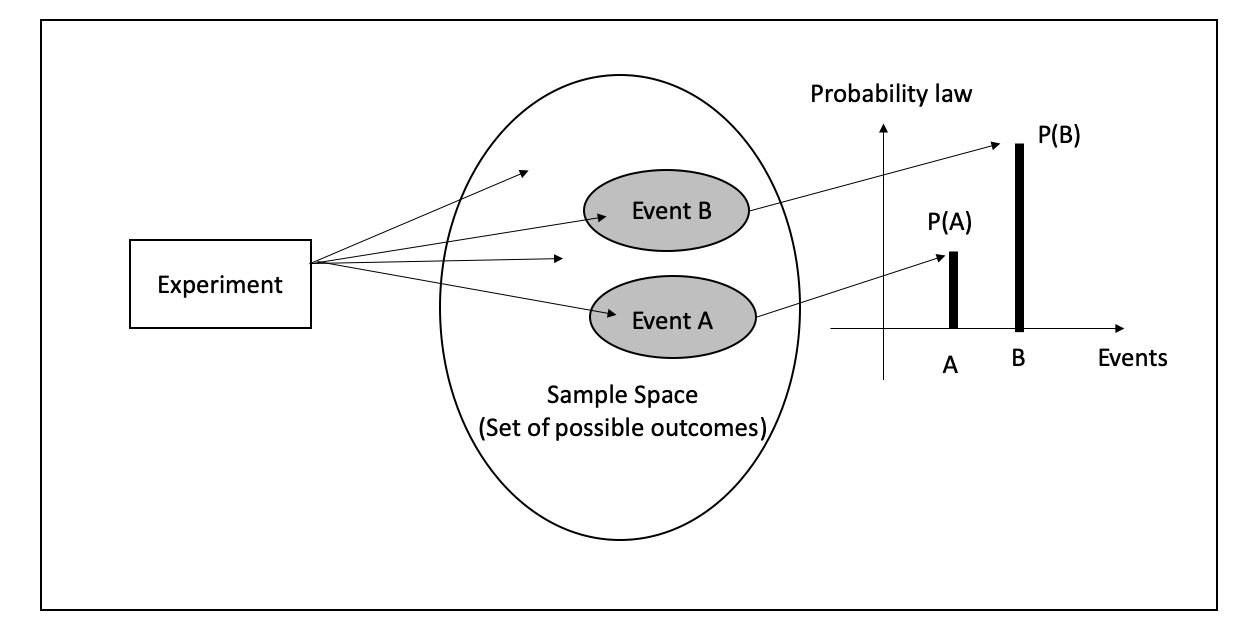
\includegraphics[width=1\linewidth]{figure/Axioms} \end{center}

\begin{itemize}
\item
  \textbf{Probability} of an event quantifies the \textbf{uncertainty}, randomness, or the possibility of occurrence the event.
\item
  The probability of event E is usually denoted by \(P(E)\).
\item
  Mathematically, the function \(P(.)\) is a set function defined from sample space \((\Omega)\) to \([0, 1]\) interval, satisfying the following properties.
\item
  These are called the \textbf{`axioms of probability'}.
\item
  \textbf{Axiom 1:} For any event \(A\), \(P(A) \geq 0\)
\item
  \textbf{Axiom 2:} \(P(\Omega) = 1\)
\item
  \textbf{Axiom 3:}

  \begin{itemize}
  \item
    \begin{enumerate}
    \def\labelenumi{(\alph{enumi})}
    \tightlist
    \item
      If \(A_1, A_2, \dots, A_k\) is a finite collection of mutually exclusive events, then \[P(A_1\cup A_2\cup \dots \cup A_k)= \sum_{i=1}^kP(A_i)\]
    \item
      If \(A_1, A_2, \dots\) is an infinite collection of mutually exclusive events, then
      \[P(A_1\cup A_2\cup \dots)= \sum_{i=1}^\infty P(A_i)\]
    \end{enumerate}
  \end{itemize}
\end{itemize}

\textbf{NOTE}

\begin{itemize}
\tightlist
\item
  Axioms 1 and 2 imply that for any event \(E\), \(0 \leq P (E) \leq 1\).
\item
  \(P (E) = 1 \iff\) the event E is certain to occur.
\item
  \(P (E) = 0 \iff\) the event E cannot occur.
\end{itemize}

\hypertarget{methods-for-determining-probability}{%
\subsection*{Methods for determining Probability}\label{methods-for-determining-probability}}
\addcontentsline{toc}{subsection}{Methods for determining Probability}

\begin{itemize}
\tightlist
\item
  There are several ways for determining the probability of events.
\item
  Usually we use the following methods to obtain the probability of events.

  \begin{itemize}
  \tightlist
  \item
    Classical method
  \item
    Relative frequency method (Empirical approach)
  \item
    Subjective method
  \item
    \textbf{Using probability models}
  \end{itemize}
\end{itemize}

\newpage

\hypertarget{random-variable}{%
\section{Random Variable}\label{random-variable}}

\begin{itemize}
\tightlist
\item
  Some sample spaces contain quantitative (numerical) outcomes, others contain qualitative outcomes.
\item
  Often it is convenient to work with sample spaces containing numerical outcomes.
\item
  A function that maps the original sample space into the real numbers is called a `random variable'.
\item
  This is more useful when the original sample space contains qualitative outcomes.
\end{itemize}

\textbf{Definition 1: Random Variable}

Let \(\Omega\) be a sample space. Let \(X\) be a function from \(\Omega\) to \(\Re\) (\emph{i.e.} \(X:\Omega \rightarrow \Re\)). Then \(X\) is called a random variable.

\begin{center}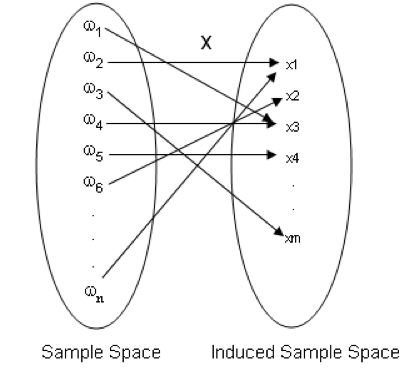
\includegraphics[width=0.5\linewidth]{figure/Ch1_F1} \end{center}

\begin{itemize}
\tightlist
\item
  A random variable assigns a real number to each outcome of a sample space.
\item
  In other words, to each outcome of an experiment or a sample point \(\omega_i\), of the sample spaces, there is a unique real number \(x_i\), known as the value of the random variable \(X\).
\item
  The range of the random variable is called the \emph{induced sample space}.
\item
  \emph{A note on notation:} Random variables will always denoted with uppercase letters and the realized values of the random variable (or its range) will be denoted by the corresponding lowercase letters. Thus, the random variable \(X\) can take the value \(x\).
\item
  Each outcome of a sample space occurs with a certain probability. Therefore, each possible value of a random variable is associated with a probability.
\item
  Any events of a sample space can be written in terms of a suitably defined random variable.
\end{itemize}

\hypertarget{types-of-random-variables}{%
\subsection{Types of Random Variables}\label{types-of-random-variables}}

\begin{itemize}
\tightlist
\item
  A random variable is of two types

  \begin{itemize}
  \tightlist
  \item
    Discrete Random Variable
  \item
    Continuous Random Variable
  \end{itemize}
\end{itemize}

\hypertarget{discrete-random-variable}{%
\subsubsection{Discrete Random Variable}\label{discrete-random-variable}}

\begin{itemize}
\tightlist
\item
  If the induced sample space is discrete, then the random variable is called a \textbf{discrete random variable}.
\end{itemize}

\emph{Example 01}
Consider the experiment of tossing a coin. Express the following events using a suitably defined random variable

\(H=\) \emph{The event of getting a head}

\(T=\) \emph{The event of getting a tail}

\begin{center}
\includegraphics[width=1\linewidth]{figure/Ch1box1-1} \end{center}

\emph{Example 02}

Consider the experiment of rolling of a die. Express the following events using a suitably defined random variable

\(A=\) \emph{The event that the number faced up is less than 5}

\(B=\) \emph{The event that the number faced up is even}

\(C=\) \emph{The event that the number faced up is 2 or 5}

\begin{center}
\includegraphics[width=1\linewidth]{figure/Ch1box2-1} \end{center}

\newpage

\emph{Example 03}

Consider the experiment of tossing a coin 10 times. Then the sample space \(\Omega\) contains \(2^{10} = 1024\) outcomes. Each outcome is a sequence of 10 H's and T's.

Express the following events in terms of a suitably defined random variable.

\(D=\) \emph{The event that the number of heads is 5}

\(E=\) \emph{The event that the number of tails is less than 4}

\begin{center}
\includegraphics[width=1\linewidth]{figure/Ch1box3-1} \end{center}

\hypertarget{continuous-random-variable}{%
\subsubsection{Continuous Random Variable}\label{continuous-random-variable}}

\begin{itemize}
\tightlist
\item
  If the induced sample space is continuous, then the random variable is called a \textbf{continuous random variable.}
\end{itemize}

\emph{Example 04}

Consider the experiment of measuring the lifetime (in hours) of a randomly selected bulb. Express the following events in terms of a suitably defined random variable.

\(F=\) \emph{The event that the lifetime is less than 300 hours}

\(G=\) \emph{The event that the lifetime is 1000 hours}

\begin{center}
\includegraphics[width=1\linewidth]{figure/Ch1box4-1} \end{center}

\hypertarget{probability-mass-function}{%
\section{Probability Mass Function}\label{probability-mass-function}}

\label{sec:pmf}

\textbf{Definition 2: Discrete density function of a discrete random variable}

If \(X\) is a discrete random variable with distinct values \(x_1, x_2, \dots, x_n, \dots,\) then the function, denoted by \(f_X(.)\) and defined by

\begin{equation}
f_X(x) =
\begin{cases} 
P(X=x) & \text{if } x=x_j, j=1,2,\dots,n,\dots\\
0 & \text{if } x \neq x_j
\end{cases}
\end{equation}

is defined to be the discrete density function of \(X\).

\begin{itemize}
\tightlist
\item
  The values of a discrete random variable are often called \emph{mass points.}
\item
  \(f_X(x)\) denotes the \emph{mass} associated with the \emph{mass point} \(x_j\).
\item
  \textbf{\emph{Probability mass function}} \emph{discrete frequency function} and \emph{probability function} are other terms used in place of \emph{discrete density function}
\item
  Probability function gives the measure of probability for different values of \(X\).
\end{itemize}

\hypertarget{properties-of-a-probability-mass-function}{%
\subsection{Properties of a Probability Mass Function}\label{properties-of-a-probability-mass-function}}

\begin{itemize}
\tightlist
\item
  Let \(X\) be a discrete random variable with probability mass function \(f_X(x)\). Then,
\end{itemize}

\begin{enumerate}
\def\labelenumi{\arabic{enumi}.}
\tightlist
\item
  For any \(x\in \Re\), \(0\leq f_X(x) \leq 1.\)
\item
  Let \(E\) be an event and \(I= \{X(\omega):\omega \in E\}.\) Then \(P(E) = P(X\in I) = \sum_{x \in I}f_X(x).\)
\item
  Let \(R = \{X(\omega):\omega \in \Omega\}.\) Then \(\sum_{x\in \Re} f_X(x) = 1.\)
\end{enumerate}

\hypertarget{representations-of-probability-mass-functions}{%
\subsection{Representations of Probability Mass Functions}\label{representations-of-probability-mass-functions}}

\emph{Example 05}

Consider the experiment of tossing a fair coin. Let

\begin{equation}
X =
\begin{cases} 
0 & \text{if the outcome is a Tail }\\
1 & \text{if the outcome is a Head}
\end{cases}
\end{equation}

Find the probability mass function of \(X\). Is \(X\) discrete or continuous?

\hypertarget{using-a-table}{%
\subsubsection{Using a table}\label{using-a-table}}

\begin{center}
\includegraphics[width=1\linewidth]{figure/Ch1box5-1} \end{center}

\hypertarget{using-a-function}{%
\subsubsection{Using a function}\label{using-a-function}}

\begin{center}
\includegraphics[width=1\linewidth]{figure/Ch1box6-1} \end{center}

\hypertarget{using-a-graph}{%
\subsubsection{Using a graph}\label{using-a-graph}}

\begin{center}
\includegraphics[width=1\linewidth]{figure/Ch1box7-1} \end{center}

\hypertarget{probability-density-function}{%
\section{Probability Density Function}\label{probability-density-function}}

\begin{itemize}
\item
  Let \(X\) be a continuous random variable.
\item
  Then, it is not possible to define a pmf \(f_x\) with properties mentioned in Section \ref{sec:pmf}. \textbf{Why?}
\item
  Instead, we can find a function \(f_x\) with the some different properties.
\item
  Probability density function (pdf) of a continuous random variable is a function that describes the relative likelihood for this random variable to occur at a given point.
\end{itemize}

\hypertarget{properties-of-a-probability-density-function}{%
\subsection{Properties of a Probability Density Function}\label{properties-of-a-probability-density-function}}

\label{sec:pdfproperties}

Let \(X\) be a continuous random variable with probability density function \(f_x\). Then,

\begin{enumerate}
\def\labelenumi{\arabic{enumi}.}
\tightlist
\item
  For any \(x\in \Re\), \(f_X(x) \geq0\).
\item
  Let \(E\) be an event and \(I= \{X(\omega):\omega \in E\}.\) Then \(P(E) = P(X\in I) = \int_If_X(x)dx.\)
\item
  Let \(R = \{X(\omega):\omega \in \Omega\}.\) Then \(\int_\Re f_X(x)dx= 1.\)
\end{enumerate}

\hypertarget{existence-of-pdf}{%
\subsection{Existence of pdf}\label{existence-of-pdf}}

\begin{itemize}
\tightlist
\item
  To see the existence of such a function, consider a continuous random variable \(X\),
\item
  Suppose that we have a very large number of observations, \(N\), of \(X\), measured to high accuracy (large number of decimal places).
\item
  consider the following grouped frequency table and the histogram constructed from those data.
\item
  The height of the bar on a class interval of this histogram is equal to the relative frequency per unit in that class interval.
\end{itemize}

\begin{longtable}[]{@{}lllll@{}}
\toprule
Interval & Class boundaries & Class frequency & Height of the bar & Area of the bar\tabularnewline
\midrule
\endhead
\(I_1\) & \(x_1 -\delta x/2, x_1+\delta x/2\) & \(n_1\) & \(\frac{n_1}{\delta x*N}\) & \(\frac{n1}{N}\)\tabularnewline
\(I_2\) & \(x_2 -\delta x/2, x_2+\delta x/2\) & \(n_2\) & \(\frac{n_2}{\delta x*N}\) & \(\frac{n2}{N}\)\tabularnewline
\(\vdots\) & \(\vdots\) & \(\vdots\) & \(\vdots\) & \(\vdots\)\tabularnewline
\(I_k\) & \(x_k -\delta x/2, x_k+\delta x/2\) & \(n_k\) & \(\frac{n_k}{\delta x*N}\) & \(\frac{nk}{N}\)\tabularnewline
Total & & & &\tabularnewline
\bottomrule
\end{longtable}

\begin{figure}

{\centering 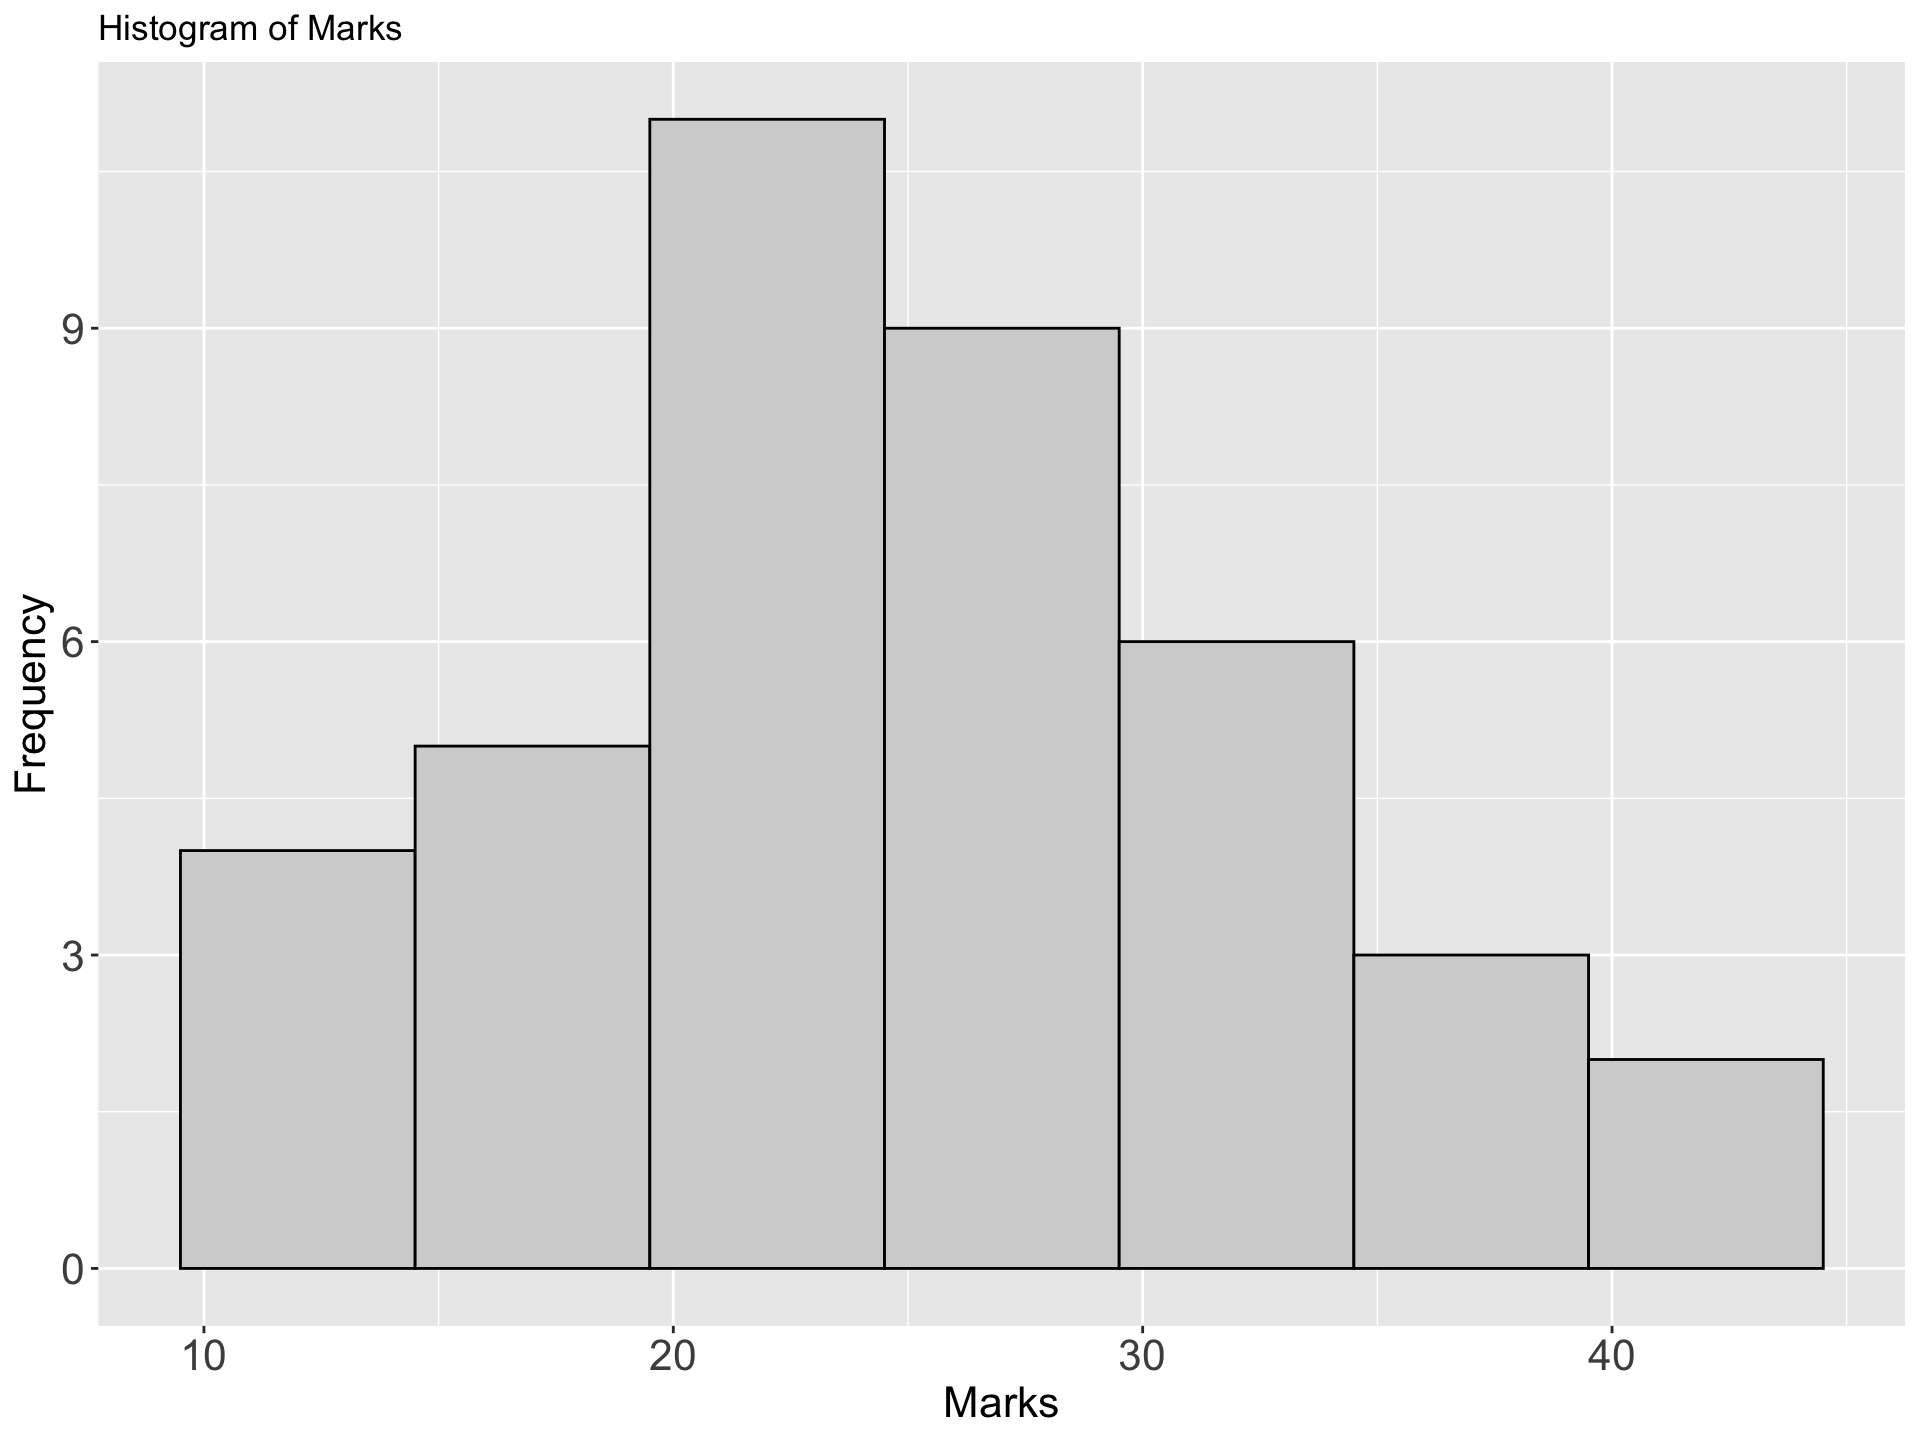
\includegraphics{figure/hist-1} 

}

\caption{Histograms with different class intervals and a possible model for the pdf}\label{fig:hist}
\end{figure}

\begin{itemize}
\tightlist
\item
  Then, for the \(i^{th}\) interval,
\end{itemize}

\[P(x_i - \frac{\delta x}{2} \leq X \leq x_i + \frac{\delta x}{2}) \approx \text{Area of the bar} \]
and therefore

\[\text{Height of the bar} \approx \frac{\text{Area of the bar}}{\delta x} \approx \frac{ P(x_i - \frac{\delta x}{2} \leq X \leq x_i + \frac{\delta x}{2})}{\delta x}  \]

\begin{itemize}
\item
  Therefore, the height of a bar represents the \emph{probability density} in that class interval.
\item
  When \(\delta x \rightarrow0\), it will allow us to approximate the histogram by a smooth curve as in Figure \ref{fig:hist} (d).
\item
  As the area under each histogram is 1, the area under the curve is also 1
\item
  For any point \(x\),
\end{itemize}

\[\text{The height of the curve} \approx \lim \limits_{\delta x \to 0} \frac{P(x_i-\frac{\delta x}{2} \leq X \leq x_i+\frac{\delta x}{2})}{\delta x} \]

will represent the \textbf{the probability density at point} \(x\).

\begin{itemize}
\item
  Let the above smooth curve be denoted by \(f_X\).
\item
  Then, \(f_X\) has the properties mentioned in Section \ref{sec:pdfproperties}.
\item
  The function is called the \textbf{probability density function of}
  \(X\).
\item
  \textbf{NOTE} Here \(f_X(x)\) represents \textbf{Probability density} \emph{at point} \(x\). Not \emph{Probability at point} \(x\).
\end{itemize}

\hypertarget{calculation-of-probability-using-pdf}{%
\subsection{Calculation of Probability using pdf}\label{calculation-of-probability-using-pdf}}

\begin{itemize}
\tightlist
\item
  Let \(c,d \in \Re\) such that \(c\leq d\). Then,
\end{itemize}

\[P(c\leq X \leq d) = \int_c^d f_X(x)dx\]

\begin{figure}

{\centering 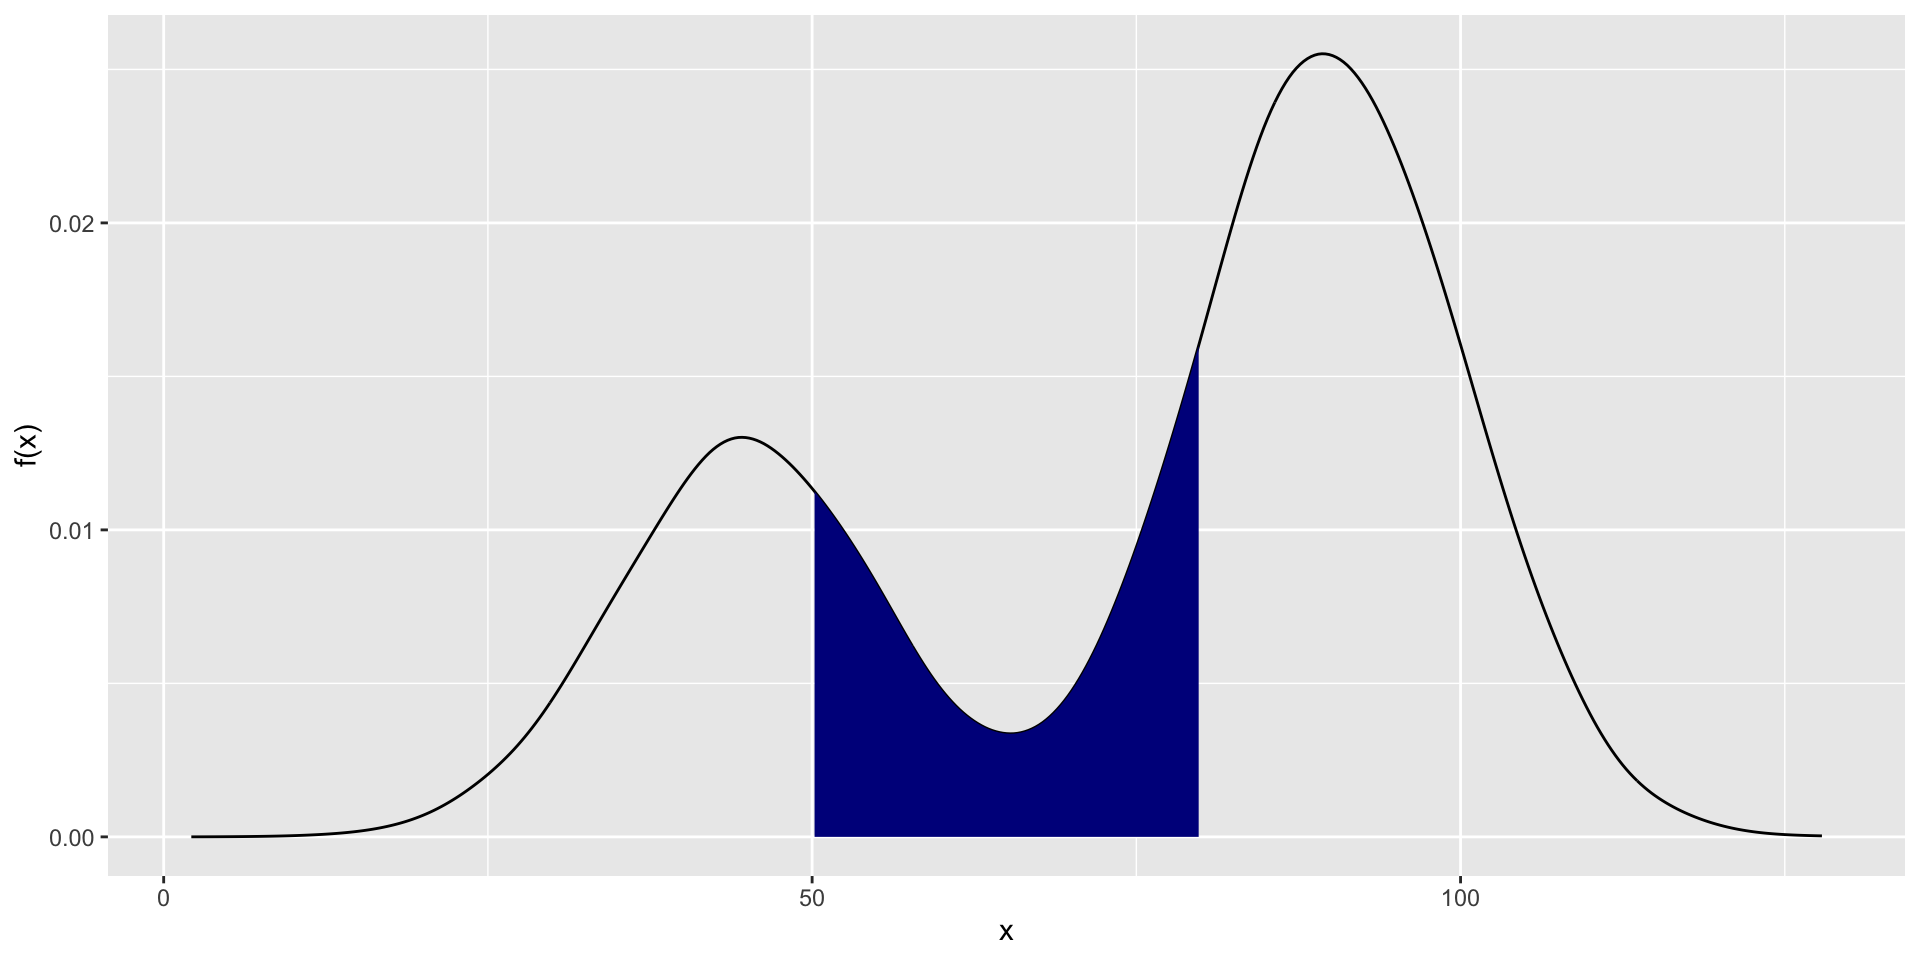
\includegraphics{figure/hist2-1} 

}

\caption{$P(c\leq x \leq d = \int_c^d f_X(x)dx$}\label{fig:hist2}
\end{figure}

\begin{itemize}
\tightlist
\item
  \textbf{NOTE:} if \(X\) is a continuous random variable with the p.d.f \(f_X\), then for any \(k \in \Re\),
\end{itemize}

\[P(X=k) = P(k\leq X\leq k)=\int_k^kf_X(x)dx = 0\]

\begin{itemize}
\tightlist
\item
  Therefore, for a continuous random variable \(X\),
  \[P(c<X<d) = P(c\leq X<d) =  P(c < X\leq d)=  P(c \leq X\leq d)= \int_c^df_X(x)dx\]
\end{itemize}

\hypertarget{cumulative-distribution-function}{%
\section{Cumulative Distribution Function}\label{cumulative-distribution-function}}

\begin{itemize}
\tightlist
\item
  There are many problems in which it is of interest to know the probability that the values of a random variable is less than or equal to some real number \(x\).
\end{itemize}

\textbf{Definition 3: Cumulative distribution function}

The \emph{cumulative distibution function} or \(cdf\) of a random variable \(X\), denoted by \(F_X(x)\), is defined by

\[F_x(x) = P(X\leq x), \text{ for all } x \]

\begin{itemize}
\tightlist
\item
  Therefore, if \(X\) is a discrete random variable, the cdf is given by,
\end{itemize}

\[F_X(x)=\sum_{t\leq x}f_X(t), \text{ } -\infty < x<\infty\]

where \(f_X(t)\) is the value of the pmf of \(X\) at \(t\).

\hypertarget{relationship-between-cdf-and-pdf}{%
\subsection{Relationship between cdf and pdf}\label{relationship-between-cdf-and-pdf}}

\begin{itemize}
\tightlist
\item
  If \(X\) is a continuous random variable, the cdf is given by,
\end{itemize}

\[F_X(x) = \int_{-\infty}^{x}f_X(t)dt \text{  } -\infty <x<\infty\]
where \(f_X(t)\) is the value of the pdf of \(X\) at \(t\). (Here \(t\) is a dummy integration variable).

\begin{itemize}
\tightlist
\item
  Conversely,
\end{itemize}

\[f_X(x)= \frac{dF_X(x)}{dx}\]

\emph{Example 06}

An owner of a software engineering company is interested in knowing how many years his employees stay with his company. Let \(X\) be the number of years an employee will stay with the company. Over the years, he has established the following probability distribution:

\newpage

\begin{longtable}[]{@{}llllllll@{}}
\toprule
\(x\) & 1 & 2 & 3 & 4 & 5 & 6 & 7\tabularnewline
\midrule
\endhead
\(f_X(x) = P(X=x)\) & 0.1 & 0.05 & 0.1 & ? & 0.3 & 0.2 & 0.1\tabularnewline
\bottomrule
\end{longtable}

\begin{enumerate}
\def\labelenumi{\arabic{enumi}.}
\tightlist
\item
  Find \(f_X(4)\)
\end{enumerate}

\begin{center}
\includegraphics[width=1\linewidth]{figure/Ch1box8-1} \end{center}

\begin{enumerate}
\def\labelenumi{\arabic{enumi}.}
\setcounter{enumi}{1}
\tightlist
\item
  Find \(P(X<4)\)
\end{enumerate}

\begin{center}
\includegraphics[width=1\linewidth]{figure/Ch1box9-1} \end{center}

\begin{enumerate}
\def\labelenumi{\arabic{enumi}.}
\setcounter{enumi}{2}
\tightlist
\item
  Find \(P(X\leq4)\)
\end{enumerate}

\begin{center}
\includegraphics[width=1\linewidth]{figure/Ch1box10-1} \end{center}

\begin{enumerate}
\def\labelenumi{\arabic{enumi}.}
\setcounter{enumi}{3}
\tightlist
\item
  Draw the probability mass function of \(X\)
\end{enumerate}

\begin{center}
\includegraphics[width=1\linewidth]{figure/Ch1box11-1} \end{center}

\begin{enumerate}
\def\labelenumi{\arabic{enumi}.}
\setcounter{enumi}{4}
\tightlist
\item
  Draw the cumulative distribution function of \(X\)
\end{enumerate}

\begin{center}
\includegraphics[width=1\linewidth]{figure/Ch1box12-1} \end{center}

\begin{center}
\includegraphics[width=1\linewidth]{figure/Ch1box13-1} \end{center}

\hypertarget{properties-of-a-cumulative-distribution-function-of-a-discrete-random-variable}{%
\subsection{Properties of a cumulative distribution function of a Discrete random variable}\label{properties-of-a-cumulative-distribution-function-of-a-discrete-random-variable}}

\emph{Example 07}

\begin{equation}
f_X(x) =
\begin{cases} 
\frac{1}{25}x & 0\leq x < 5\\
\frac{2}{5}- \frac{1}{25}x & 5\leq x \leq 10\\
0 & \text{otherwise}
\end{cases}
\end{equation}

\begin{enumerate}
\def\labelenumi{\arabic{enumi}.}
\tightlist
\item
  Find the CDF of \(X\)
\item
  Find \(P(X\leq 8)\)
\item
  Find \(P(3\leq X\leq 8)\)
\end{enumerate}

\newpage

\begin{enumerate}
\def\labelenumi{\arabic{enumi}.}
\item
\end{enumerate}

\newpage

\hypertarget{expectations-and-moments}{%
\section{Expectations and Moments}\label{expectations-and-moments}}

\hypertarget{expectation}{%
\subsection{Expectation}\label{expectation}}

\begin{itemize}
\item
  The expected value, or expectation of a random variable is merely its average value.
\item
  By weighting the values of the random variable according to the probability distribution, we can obtain a number that summarizes a typical or expected value of an observation of the random variable.
\end{itemize}

\textbf{Definition 4: Expected value}

Let \(X\) be a random variable. The \emph{expected value} or \emph{mean} of a random variable \(g(X)\), denoted by \(E[g(x)],\) is

\begin{equation}
E[g(x)] =
\begin{cases} 
\sum_{x}g(x) f_X(x) & \text{if } X \text{ is a discrete random variable with pmf }  f_X(x) \\
\int_x g(x) f_X(x)dx & \text{if } X \text{ is a continuous random variable with pdf }  f_X(x)
\end{cases}
\end{equation}

\begin{itemize}
\item
  The mean of a random variable gives a measure of \emph{central location} of the density of \(X\).
\item
  The process of taking expectations is a linear operation.
\item
  For any constants \(a\) and \(b\),
  \[E(aX+b) = aE(X)+b\]
\end{itemize}

\hypertarget{properties-of-expected-value}{%
\subsubsection{Properties of expected value}\label{properties-of-expected-value}}

\textbf{Theorem}

\begin{enumerate}
\def\labelenumi{\alph{enumi}.}
\tightlist
\item
  \(E(c) = c\) for a constant \(c\)
\item
  \(E[cg(X)] = cE[g(X)]\) for a constant \(c\)
\item
  \(E[c_1g_1(X)+c_2g_2(X)]= c_1E[g_1(X)]+c_2E[g_2(X)]\)
\item
  If \(g_1(x) \geq 0\) for all \(x\), then \(E[g_1(X)] \geq 0\)
\item
  If \(g_1(x) \geq g_2(x)\) for all \(x\), then \(E[g_1(X)] \geq E[g_2(X)]\)
\item
  If \(a\leq g_1(x) \leq b\) for all \(x\), then \(a\leq E[g_1(X)] \leq b\)
\item
  If \(X\) and \(Y\) are two \textbf{independent} random variables, then \(E(X \times Y) = E(X)\times E(Y)\)
\end{enumerate}

\emph{Example 08}

Random variable \(X\) has the following pmf

\begin{equation}
f_X(x) =
\begin{cases} 
0.2 &  x =2\\
0.3 &  x =4\\
0.4 &  x =5\\
0.1 &  x =7
\end{cases}
\end{equation}

\begin{enumerate}
\def\labelenumi{\arabic{enumi}.}
\tightlist
\item
  Find \(E(X)\)
\item
  Find \(E(X^2)\)
\item
  Find \(E\left( \frac{1}{X}\right)\)
\item
  Find \(E(2X+3X^2-5)\)
\end{enumerate}

\begin{center}
\includegraphics[width=1\linewidth]{figure/Ch1box15-1} \end{center}

\newpage

\hypertarget{moments}{%
\subsection{Moments}\label{moments}}

\begin{itemize}
\tightlist
\item
  The various moments of a distribution are an important class of expectation
\end{itemize}

\textbf{Definition 5: Moments}

If \(X\) is a random variable, the \(r\)\emph{th moment of} \(X\), usually denoted by \(\mu_r^\prime,\) is defined as

\[\mu_r^\prime = E(X^r).\]

if the expectation exists.

\begin{itemize}
\tightlist
\item
  Note that \(\mu_1^\prime = E(X)= \mu,\) the mean of \(X\).
\end{itemize}

\textbf{Definition 6: Central moments}

If \(X\) is a random variable, the \(r\)\emph{th central moment of} \(X\) \emph{about} \(a\) is defined as \(E[(x-a)^r]\).

If \(a= E(X) = \mu,\) we have the \(r\)\emph{th central moment of} \(X\), \emph{about} \(E(X)\), denoted by \(\mu_r,\) which is
\[\mu_r=E[(X-E(X))^r] = E[(X-\mu)^r] .\]

\begin{itemize}
\tightlist
\item
  Find \(\mu_1\)
\end{itemize}

\newpage

\textbf{Definition 7: Variance}

If \(X\) is a random variable, \(Var(X)= E[(X-E(X))^2]= E(X^2) - [E(X)]^2\) provided \(E(X^2)\) exists.

\begin{center}
\includegraphics[width=1\linewidth]{figure/Ch1box16-1} \end{center}

\begin{itemize}
\item
  The \emph{variance} of a random variable \(X\) is its second central moment, \(Var(X) = E[(X-E(X))^2]= E[(X-\mu)^2]\)
\item
  The positive square root of \(Var(X)\) is the \emph{standard deviation} of \(X\)
\end{itemize}

\begin{itemize}
\item
  The \emph{variance} of a random variable gives a measure of the degree of spread of a distribution around its mean.
\item
  Let \(X\) be a random variable, and let \(\mu\) be \(E(X).\) the \emph{variance} of \(X\), denoted by \(\sigma^2\) of \(Var(X),\) is defined by
\end{itemize}

\begin{equation}
Var(X) =
\begin{cases} 
\sum_{x}(x-\mu)^2f_X(x) & \text{if } X \text{ is  discrete with mass points }  x_!, x_2, \dots, x_j\dots \\
\int_x (x-\mu)^2 f_X(x)dx & \text{if } X \text{ is continuous with probability density function }  f_X(x)
\end{cases}
\end{equation}

\hypertarget{properties-of-variance-of-a-random-variable}{%
\subsubsection{Properties of variance of a random variable}\label{properties-of-variance-of-a-random-variable}}

\textbf{Theorem}

\begin{enumerate}
\def\labelenumi{\alph{enumi}.}
\tightlist
\item
  If \(c\) is a constant, then \(V(cX) = c^2V(X)\)
\item
  \(V(c) = 0\), Variance of a constant is zero.
\item
  If \(X\) is a random variable and \(c\) is a constant, then \(V(c+X) = V(X)\)
\item
  If \(a\) and \(b\) are constants, then \(V(aX+b)= a^2V(X)\)
\item
  If \(X\) and \(Y\) are two independent random variables, then

  \begin{enumerate}
  \def\labelenumii{\roman{enumii}.}
  \tightlist
  \item
    \(V(X+Y) = V(X) + V(Y)\)
  \item
    \(V(X-Y) = V(X) + V(Y)\)
  \end{enumerate}
\end{enumerate}

\begin{center}
\includegraphics[width=1\linewidth]{figure/Ch1box14-1} \end{center}

\newpage

\hypertarget{models-for-discrete-distributions}{%
\section{Models for Discrete Distributions}\label{models-for-discrete-distributions}}

\hypertarget{discrete-uniform-distribution}{%
\subsection{Discrete Uniform Distribution}\label{discrete-uniform-distribution}}

A random variable \(X\) has a \emph{discrete uniform} \((1, N)\) distribution if
\[f_X(x)= P(X=x)=\frac{1}{N}, \;\; x=1,2,\dots, N\]
where \(N\) is a specified integer.

\begin{itemize}
\item
  The distribution puts equal mass on each of the outcomes \(1,2,\dots, N.\)
\item
  If \(X\) ha s a discrete uniform distribution, then \(E(X) = (N+1)/2\) and \(Var(X) = (N^2-1)/12.\)
\end{itemize}

\hypertarget{bernoulli-distribution}{%
\subsection{Bernoulli Distribution}\label{bernoulli-distribution}}

\textbf{Bernoulli Trial}

A random experiment of which the outcome can be classified into two categories is called a \emph{Bernoulli trial}

\begin{itemize}
\item
  In general, the results of a Bernoulli Trial are called `success' and `failure'. We denote these results by \(S\) and \(F\), respectively.
\item
  Consider a Bernoulli trial. Let
\end{itemize}

\begin{equation}
X=
\begin{cases} 
0 & \text{if the Bernoulli trial results in a failure } \\
1 & \text{if the Bernoulli trial results in a success} 
\end{cases}
\end{equation}

\begin{itemize}
\item
  Suppose that the probability of a `'success' in any Bernoulli trial is \(\theta.\)
\item
  Then \(X\) is said to have a Bernoulli distribution with probability mass function
\end{itemize}

\(f_X(x)= P(X=x)=\theta^x(1-\theta)^{1-x}, \;\;x=0,1\)

\begin{itemize}
\item
  This is denoted as \(X \sim Bernoulli(\theta).\)
\item
  If \(X\) has a Bernoulli distribution, then \(E(X) = \theta\) and \(Var(X) = \theta(1-\theta)\)
\end{itemize}

\hypertarget{binomial-distribution}{%
\subsection{Binomial Distribution}\label{binomial-distribution}}

\begin{itemize}
\tightlist
\item
  A random experiment with the following properties is called a `Binomial experiment'
\end{itemize}

\begin{enumerate}
\def\labelenumi{\arabic{enumi}.}
\item
  The random experiment consists of a sequence of \(n\) trials, where \(n\) is fixed in advance of the random experiment.
\item
  Each trial can result in one of the same two possible outcomes: ``success'' \((S)\) or ``failure'' \((F)\)
\item
  The trials are independent. Therefore the outcome of any particular trial does not influence the outcome of any other trial.
\item
  The probability of ``success'' is the same for each trial. Let this probability is \(\theta.\)
\end{enumerate}

\textbf{Binomial distribution}

\begin{itemize}
\tightlist
\item
  Consider a binomial experiment with \(n\) trials and probability \(\theta\) of a success.
\end{itemize}

A random variable \(X\) is defined to have a \emph{binomial distribution} if the discrete density function of \(X\) is given by
\[f_X(x)= P(X=x)= {n\choose x}\theta ^x(1-\theta)^{n-x} , \;\; x=0,1,2,\dots, n\]

\begin{itemize}
\item
  This is denoted as \(X \sim Bin(n,\theta).\)
\item
  If \(X\) has a binomial distribution, then \(E(X) = n\theta\) and \(Var(X) = n\theta(1-\theta)\)
\item
  The binomial distribution reduces to the Bernoulli distribution when \(n=1.\)
\end{itemize}

\hypertarget{geometric-distribution}{%
\subsection{Geometric Distribution}\label{geometric-distribution}}

\begin{itemize}
\item
  Consider a sequence of independent Bernoulli trials whose probability of ``success'' for each trial is \(\theta\).
\item
  Let \(X= \text{Number of failures before the first success}\)
\item
  Then, \(X\) is said to have a Geometric distribution with parameter \(\theta.\)
\item
  The probability mass function is given by
  \[f_X(x)= P(X=x)= \theta (1-\theta)^x , \;\; x=0,1,2,\dots\]
\item
  This is denoted as \(X \sim Geometric(\theta).\)
\item
  If \(X\) has a geometric distribution, then \(E(X) = (1-\theta)/\theta\) and \(Var(X) = (1-\theta)/\theta^2\)
\item
  A random variable \(X\) that has a geometric distribution is often referred to as a discrete \emph{waiting-time} random variable. It represents how long (in terms of number of failures) one has to wait for a ``success.''
\end{itemize}

\hypertarget{negative-binomial-distribution}{%
\subsection{Negative Binomial Distribution}\label{negative-binomial-distribution}}

\begin{itemize}
\item
  Consider a sequence of independent Bernoulli trials whose probability of ``success'' for each trial is \(\theta\).
\item
  Let \(X= \text{Number of failures before the rth success}\)
\item
  Then, \(X\) is said to have a Negative Binomial distribution with parameter \(\theta.\)
\item
  The probability mass function is given by
  \[f_X(x)= P(X=x)= {x+r-1\choose r-1} \theta^r (1-\theta)^x , \;\; x=0,1,2,\dots\]
\item
  This is denoted as \(X \sim negbin(r,\theta).\)
\item
  If \(X\) has a Negative Binomial distribution, then \(E(X) = r(1-\theta)/\theta\) and \(Var(X) = r(1-\theta)/\theta^2\)
\item
  If in the negative binomial distribution \(r=1\), then the negative binomial density specializes to the geometric density. 
\end{itemize}

\hypertarget{hypergeometric-distribution}{%
\subsection{Hypergeometric Distribution}\label{hypergeometric-distribution}}

\begin{itemize}
\item
  Suppose a population of size \(N\) has \(M\) individuals of a certain kind (``success'').
\item
  A sample of \(n\) items is taken from this population without replacement.
\item
  Let \(X\) be the number of successes in the sample.
\item
  Then, \(X\) is said to have a hypergeometric distribution.
\item
  The probability mass function is given by
  \[f_X(x)= P(X=x)= \frac{{M\choose x}{N-M\choose n-x}}{{N \choose n}}  , \;\; x=0,1,2,\dots, n\]
\item
  Hypergeometric distribution can be used as a model for the number of ``successes'' in a sample of size \(n\) if the sampling is done without replacement from a relatively small population.
\item
  If \(X\) has a Hypergeometric distribution, then \(E(X) = n.\frac{M}{N}\) and \(Var(X) = n\frac{M}{N}\left(1-\frac{M}{N}\right)\left(\frac{N-n}{N-1}\right)\)
\end{itemize}

\hypertarget{poisson-distribution}{%
\subsection{Poisson Distribution}\label{poisson-distribution}}

\begin{itemize}
\item
  The Poisson distribution provides a realistic probability model for the number of events in a given period of time, space, region or length.
\item
  Example:

  \begin{itemize}
  \tightlist
  \item
    The number of fatal traffic accidents per week in a given city
  \item
    The number of emails per hour coming into the company of a large business
  \item
    the number of defect per unit of some material
  \end{itemize}
\item
  Poisson distribution is suitable if the following conditions hold.

  \begin{enumerate}
  \def\labelenumi{\arabic{enumi}.}
  \tightlist
  \item
    the number of events within non-overlapping time intervals are independent.
  \item
    Let \(t\) be a fixed time point. For a small time interval \(\delta t\), the probability of exactly one event happening in the interval \([t,t+\delta t]\) is approximately proportional to the length \(\delta t\) of the interval. \emph{i.e.,}
  \end{enumerate}
\end{itemize}

\[\frac{P(\text{exactly one event in }[t,t+\delta t])}{\delta t} \to \text{a positive constant}\]
as \(\delta t \to 0.\)

\begin{enumerate}
\def\labelenumi{\arabic{enumi}.}
\setcounter{enumi}{2}
\tightlist
\item
  Let \(t\) be a fixed time point. For a small time interval \(\delta t\), the probability of more than one event happening in the interval \([t,t+\delta t]\) is negligible. \emph{i.e.,}
\end{enumerate}

\[\frac{P(\text{more than one event in }[t,t+\delta t])}{\delta t} \to 0\]
as \(\delta t \to 0.\)

\begin{itemize}
\tightlist
\item
  Let \(X\) be the number of events during a time interval.
\item
  Suppose that the average number of events during the interested time interval is \(\lambda (>0).\)
\item
  Then, the distribution of \(X\) can be modeled by a Poisson Distribution with the probability mass function,
\end{itemize}

\[f_X(x)= P(X=x)= \frac{e^{-\lambda} (\lambda)^x}{x!}  , \;\; x=0,1,2,\dots\]
- This is denoted as \(X \sim Poisson(\lambda).\)

\begin{itemize}
\item
  If \(X\) has a Poisson distribution, then \(E(X) = \lambda\) and \(Var(X) = \lambda\)
\item
  The Poisson distribution can be used for counts of some sort of a given area, space, region, volume or length as well.
\end{itemize}

\emph{Example 09}

Phone calls arrive at a switchboard at an average rate of 2.0 calls per minute.

If the number of calls in any time interval follows the Poisson distribution, then

\(X =\) number of phone calls in a given minute.
\(X \sim Poisson(\; )\)

\(Y =\) number of phone calls in a given hour.
\(Y \sim Poisson ( \;)\)

\(W =\) number of phone calls in a 15 seconds.
\(W \sim Poisson (\;)\)

\newpage

\hypertarget{models-for-continuous-distributions}{%
\section{Models for Continuous Distributions}\label{models-for-continuous-distributions}}

\hypertarget{uniform-distribution}{%
\subsection{Uniform Distribution}\label{uniform-distribution}}

\begin{itemize}
\item
  The continuous uniform distribution is defined by spreading mass uniformly over an interval \([a,b]\).
\item
  A random variable \(X\) is said to have a uniform distribution in \((a,b)\) if its probability density function is given by
  \[f_X(x) = \frac{1}{b-a};\; a\leq x\leq b\]
\item
  This is denoted as \(X\sim U(a,b)\) or \(X \sim Unif(a, b)\)
\item
  It is easy to check \(\int_a^bf(x) dx =1\).
\item
  We also have
  \[E(X) = \int_a^b\frac{x}{b-a}dx = \frac{a+b}{2}\]
\end{itemize}

\[Var(X) =  \frac{(b-a)^2}{12}\]

\begin{figure}

{\centering 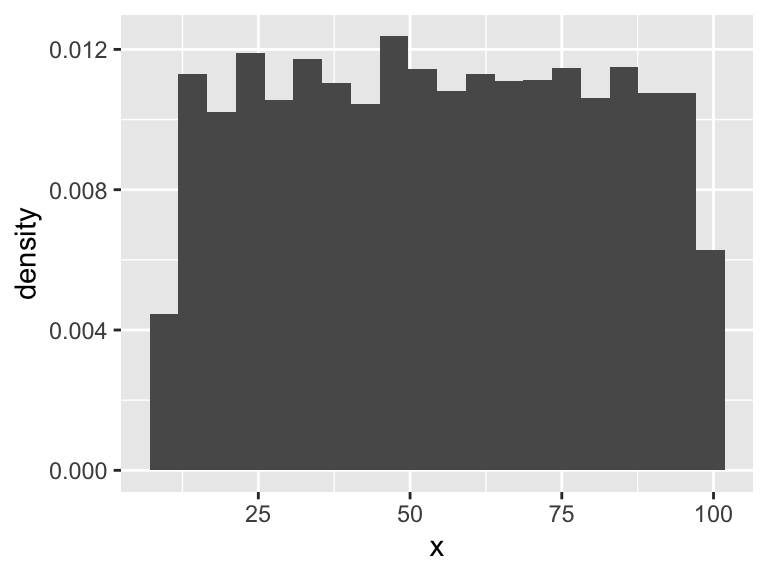
\includegraphics{figure/unif-1} 

}

\caption{Uniform probabiity density}\label{fig:unif}
\end{figure}

\hypertarget{normal-distribution-gaussian-distribution}{%
\subsection{Normal Distribution (Gaussian Distribution)}\label{normal-distribution-gaussian-distribution}}

\begin{itemize}
\item
  One commonly used bell shaped curve is called the normal distribution.
\item
  Many techniques use din applied statistics are based upon the normal distribution.
\item
  The normal distribution has two parameters, usually denoted by \(\mu\) and \(\sigma^2\), which are its mean and variance.
\item
  A random variable \(X\) is said to have a normal distribution with location parameter \(\mu\) and scale parameter \(\sigma\), if its probability density function is given by,
\end{itemize}

\[f_X(x)=f_X(x;\mu, \sigma)= \frac{1}{\sqrt{2\pi}\sigma}e^{-\frac{1}{2}\left(\frac{x-\mu}{\sigma}\right)^2};\;\; -\infty<x<\infty\]

\begin{itemize}
\item
  This is denoted by \(X \sim N(\mu, \sigma^2)\).
\item
  The normal density function is \textbf{symmetric around} the location parameter \(\mu\).
\item
  The \textbf{dispersion of the distribution} depends on the scale parameter \(\sigma\).
\item
  If \(X\) is a normal random variable, \(E(X) = \mu\) and \(Vax(X) = \sigma^2\)
\end{itemize}

\begin{figure}

{\centering 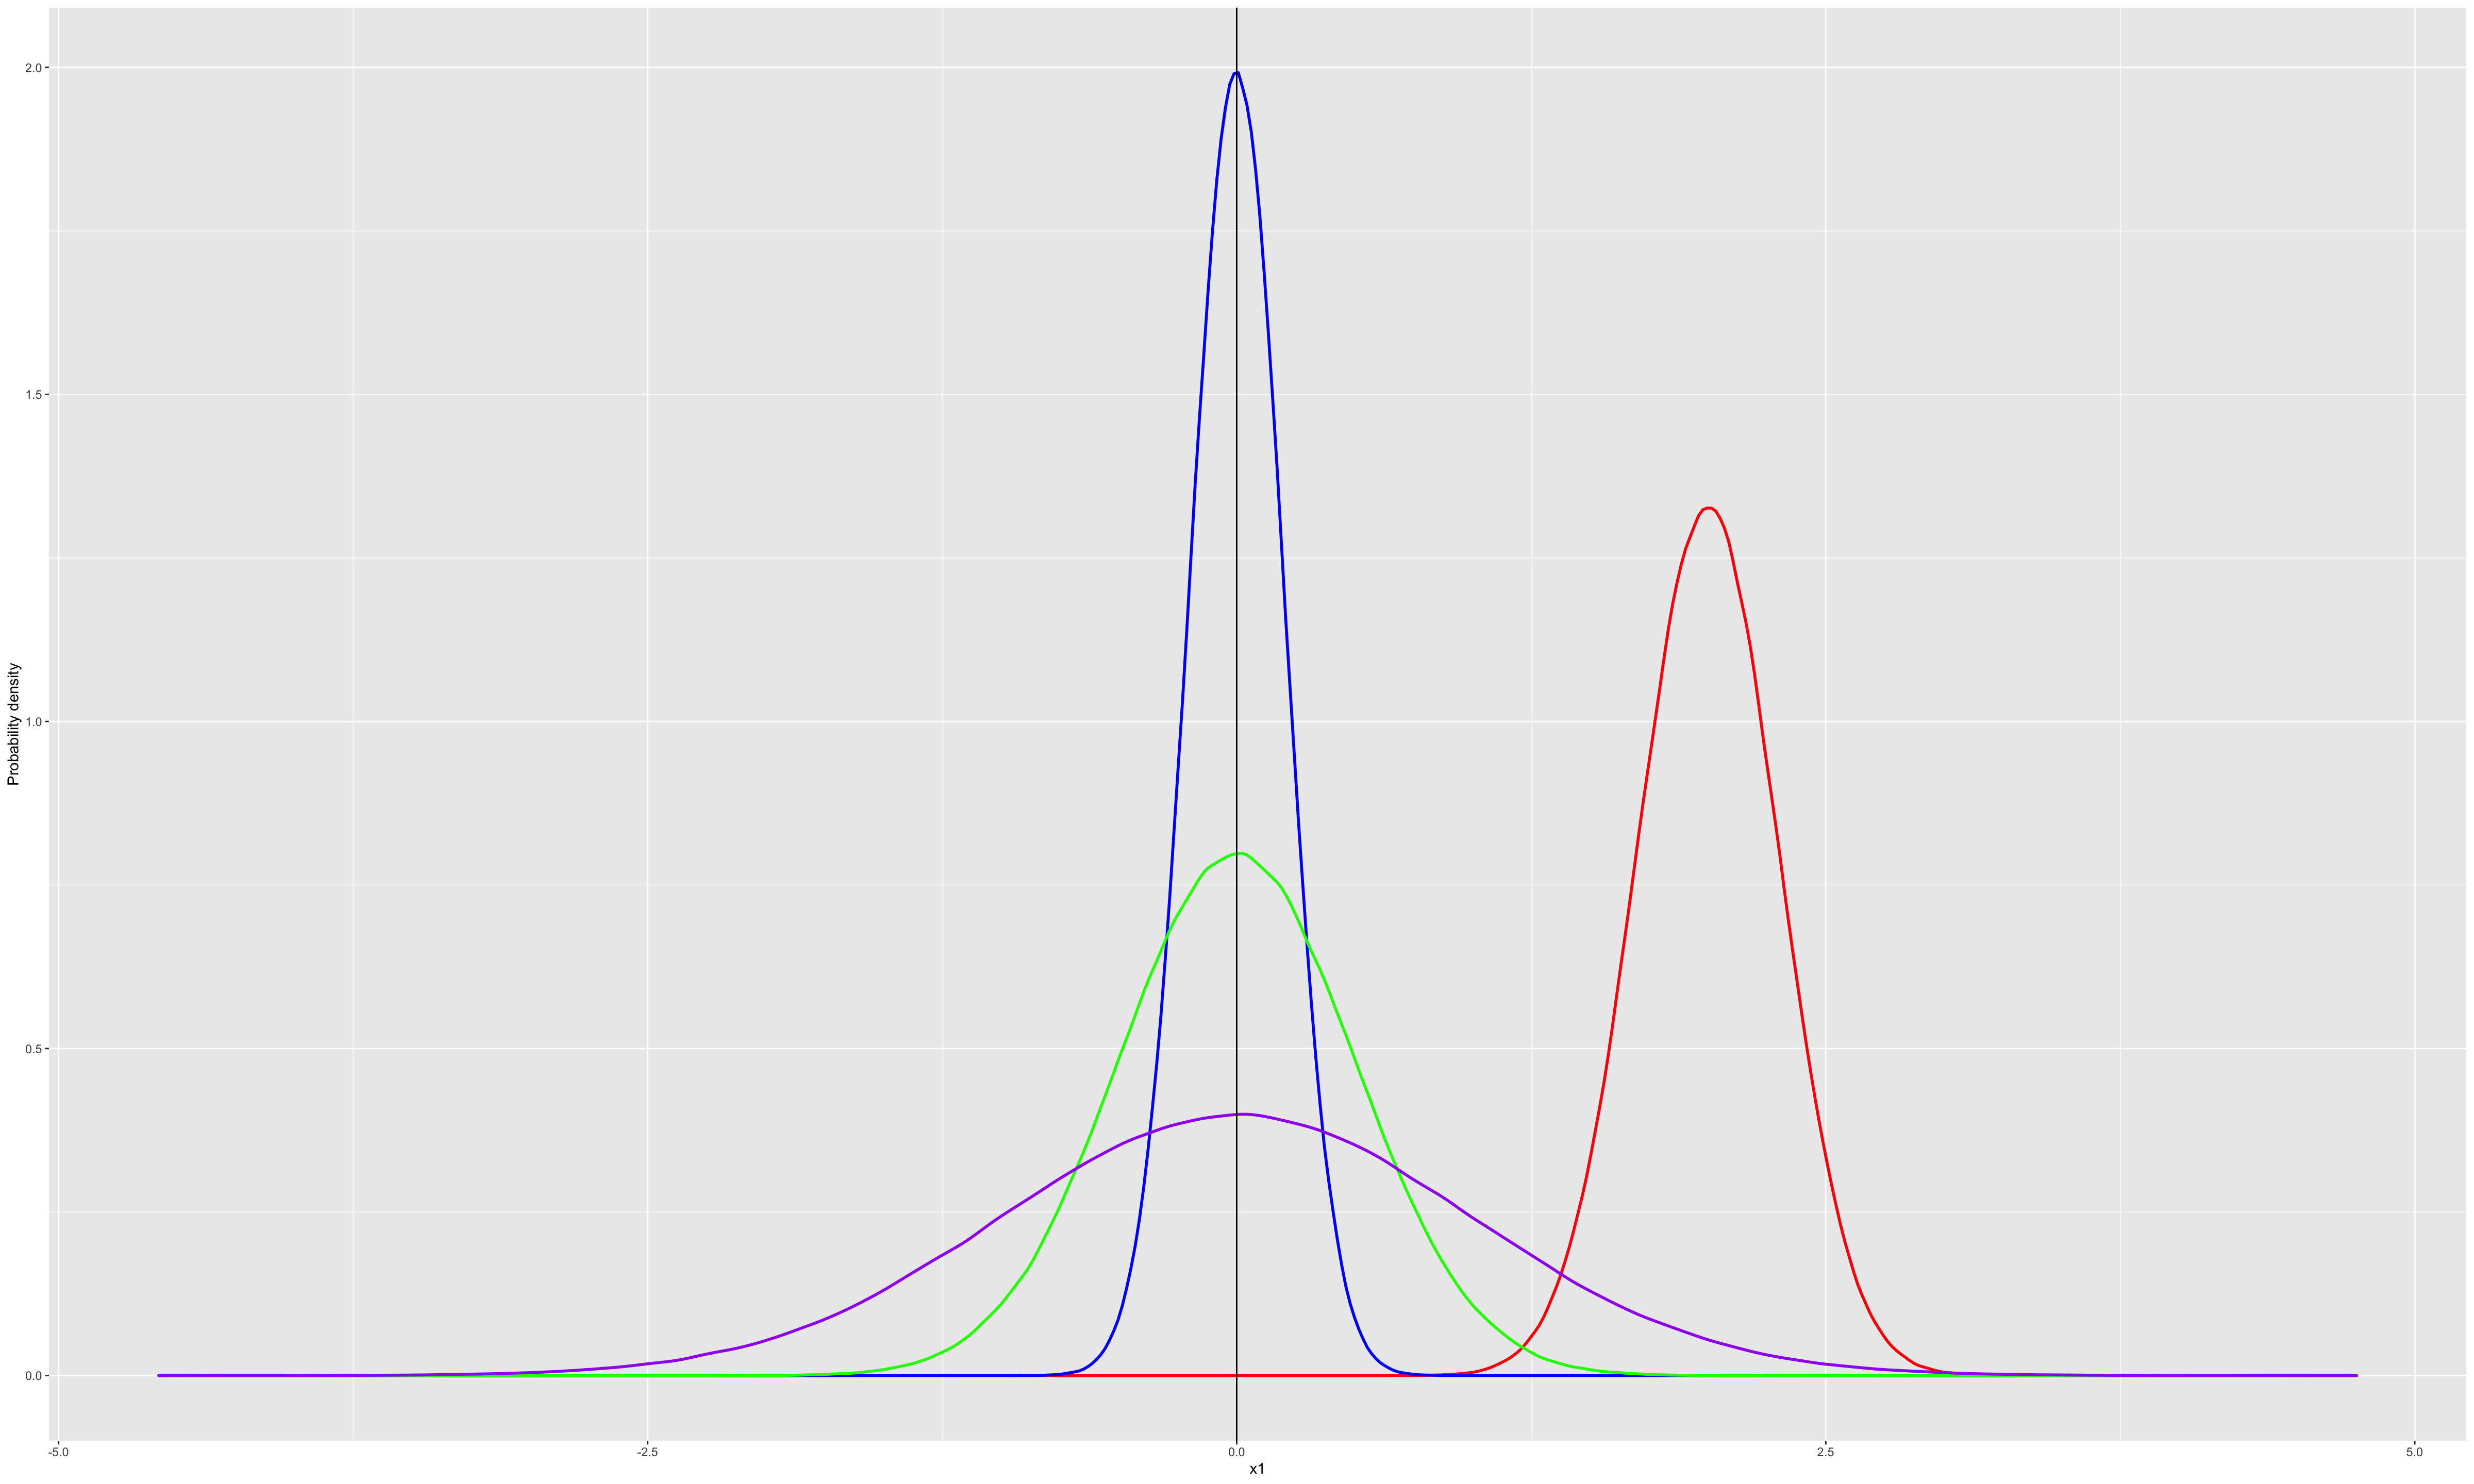
\includegraphics{figure/norm-1} 

}

\caption{Normal distribution for different $\mu$ and $\sigma$}\label{fig:norm}
\end{figure}

\begin{figure}

{\centering 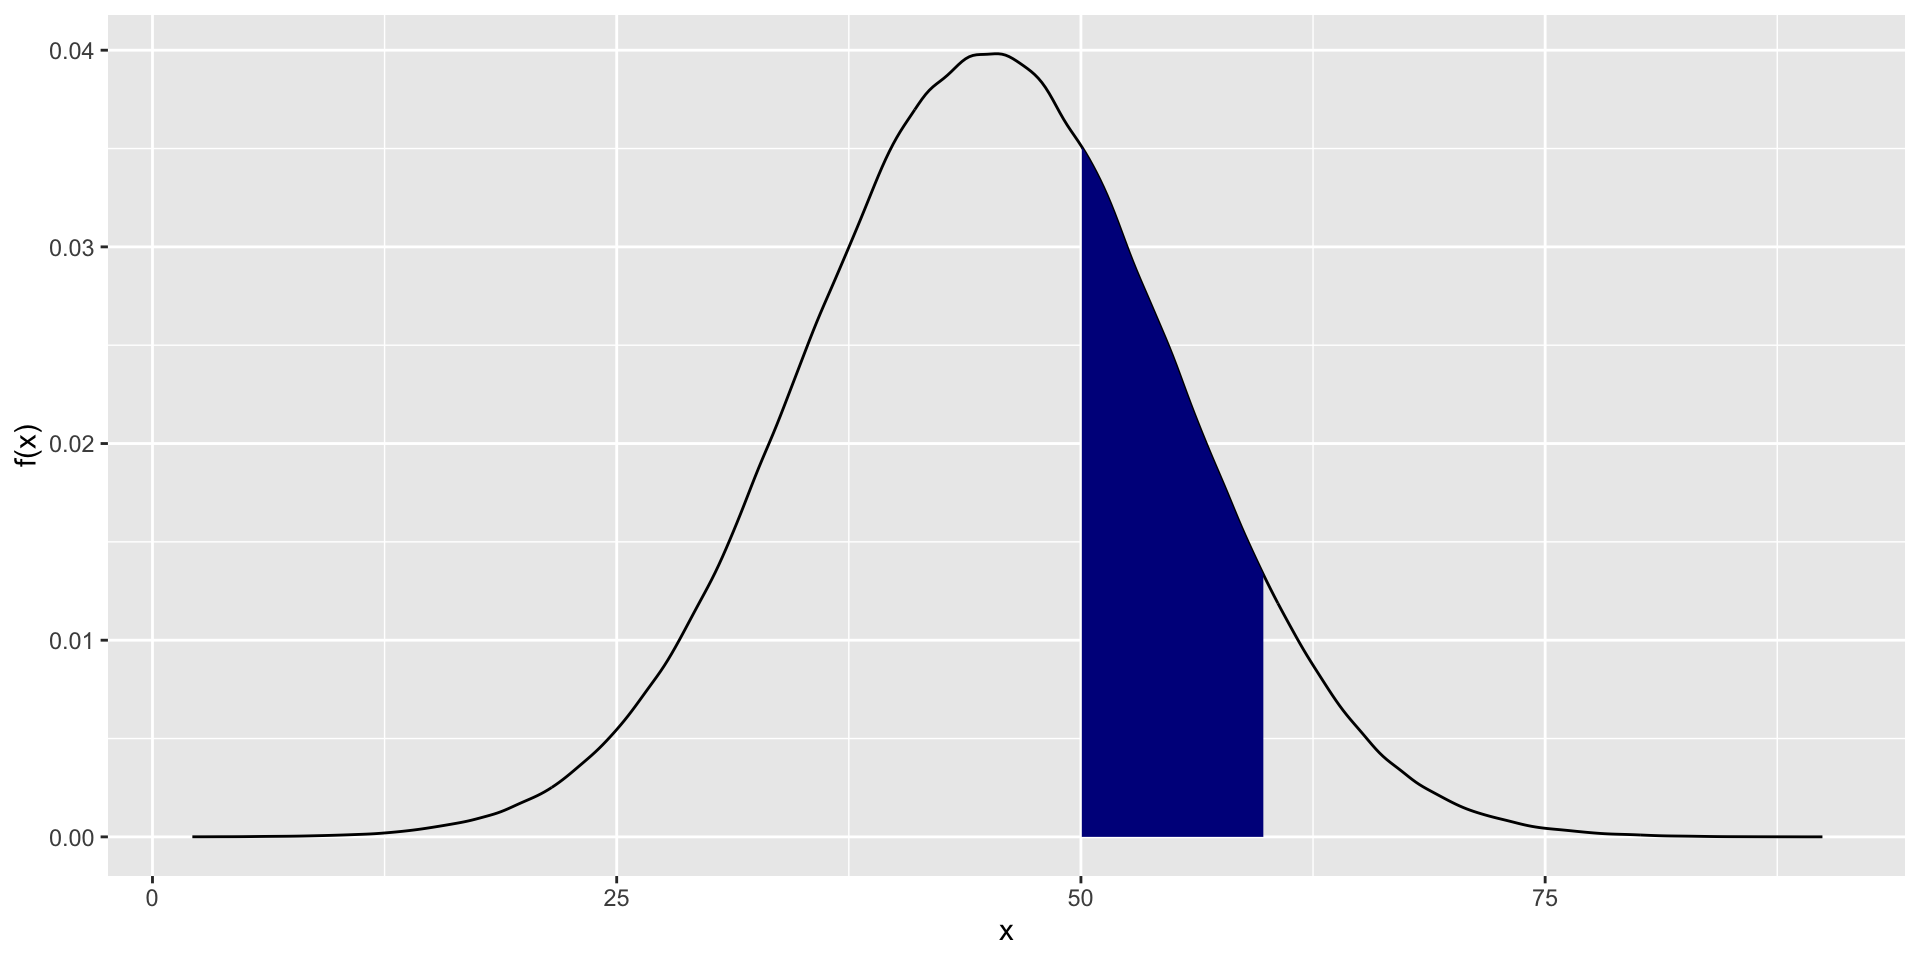
\includegraphics{figure/norm2-1} 

}

\caption{$P(a< X < b = \int_a^b f_X(x)dx$}\label{fig:norm2}
\end{figure}

\[P(a<X<b)=\int_a^b \frac{1}{\sqrt{2\pi}\sigma}e^{-\frac{1}{2}\left(\frac{x-\mu}{\sigma}\right)^2}dx\]

\begin{itemize}
\tightlist
\item
  Evaluating of this integration is somewhat tedious
\item
  When we calculate this type of probabilities of normal distribution manually, it is convenient to use a normal probability table.
\end{itemize}

\hypertarget{standard-normal-distribution}{%
\subsubsection{Standard Normal Distribution}\label{standard-normal-distribution}}

\begin{itemize}
\tightlist
\item
  Normal distribution with \(\mu =0\) and \(\sigma = 1\) is called the \textbf{standard normal distribution}.
\item
  A random variable with standard normal distribution is usually denoted by \(Z\).
\item
  The probability density function of standard normal distribution is denoted by \(\phi\)
\item
  If \(Z\sim N(0,1)\), then
\end{itemize}

\[\phi_Z(z) = \frac{1}{\sqrt{2 \pi}}e^{-\frac{1}{2}z^2};\;\; -\infty< z< \infty\]

\begin{itemize}
\tightlist
\item
  Probabilities related to Z can be found by using standard normal probability table.
\end{itemize}

\newpage

\emph{Example 10}

Let \(Z\) be a standard normal random variable. Calculate probabilities given in table below.

\begin{longtable}[]{@{}lll@{}}
\toprule
No. & Calculate this probability & Answer\tabularnewline
\midrule
\endhead
1 & \(P(Z < 0)\) &\tabularnewline
2 & \(P(Z < 2.02)\) &\tabularnewline
3 & \(P(Z > 0.95)\) &\tabularnewline
4 & \(P(Z > -1.48)\) &\tabularnewline
5 & \(P(Z < -1.76)\) &\tabularnewline
6 & \(P(Z < 1.7)\) &\tabularnewline
7 & \(P(Z < -0.33)\) &\tabularnewline
8 & \(P(0.94 < Z < 2.41)\) &\tabularnewline
9 & \(P(-2.41 < Z < -0.94)\) &\tabularnewline
10 & \(P(-2.96 < Z < 1.05)\) &\tabularnewline
\bottomrule
\end{longtable}

\newpage

Example contd\ldots{}

\newpage

\textbf{Cumulative Standard Normal Distribution}

\begin{center}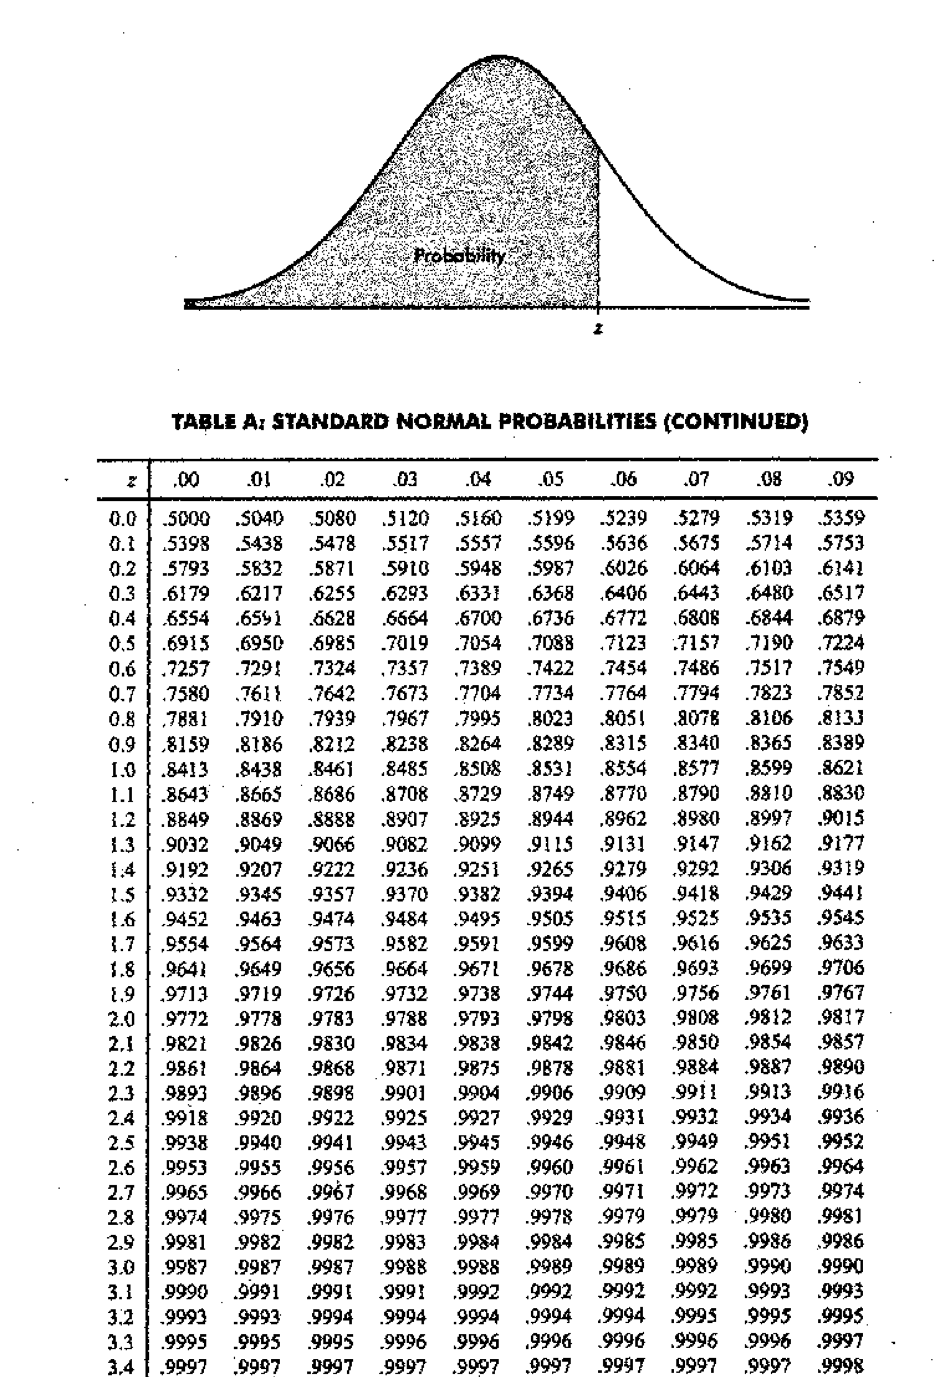
\includegraphics[width=1\linewidth]{figure/ztable} \end{center}

\newpage

\(Z_\alpha\) \textbf{Notation}

\begin{itemize}
\tightlist
\item
  \(Z_\alpha\) denotes the value such that \(P(Z\geq Z_\alpha) = \alpha\)
\item
  Here \(\alpha\) represents a probability.
\item
  Therfore \(0\leq \alpha \leq 1\)
\end{itemize}

\emph{Example 11}

Find \(Z_{0.025}\)''

\begin{figure}

{\centering 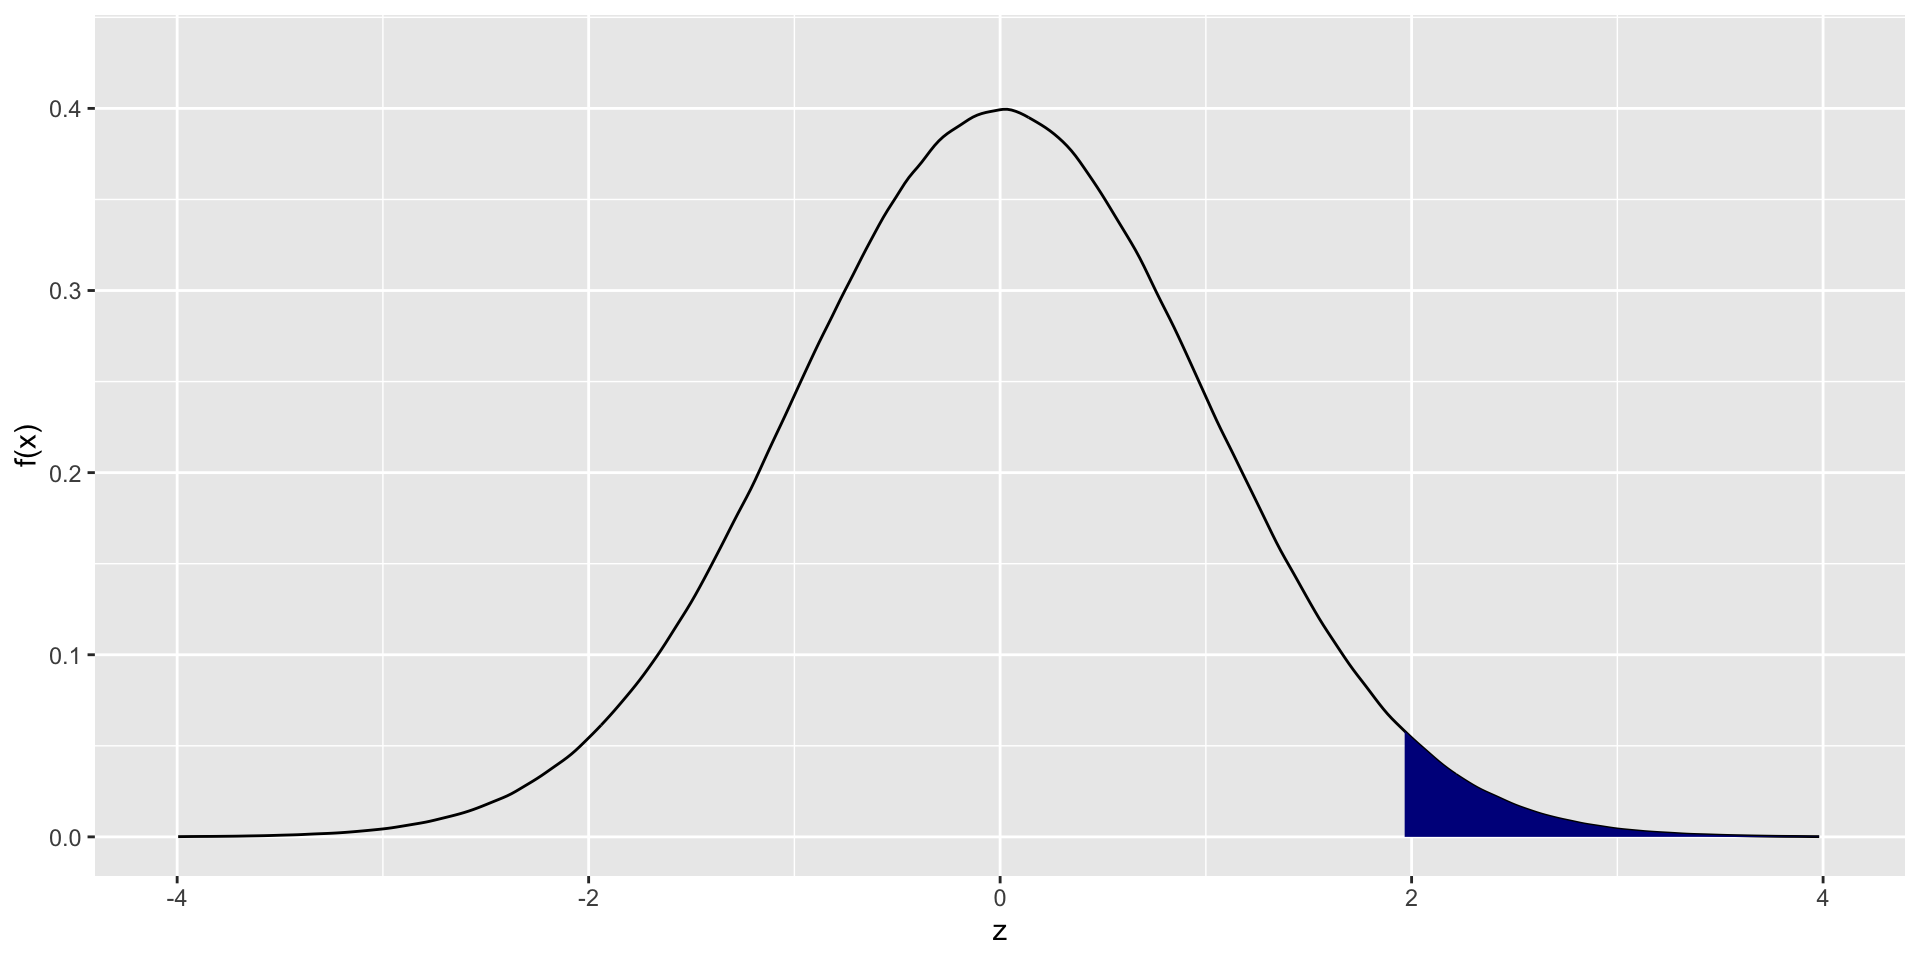
\includegraphics{figure/norm3-1} 

}

\caption{$P(a< X < b = \int_a^b f_X(x)dx$}\label{fig:norm3}
\end{figure}

\emph{Example 12}

Find the following values

\begin{enumerate}
\def\labelenumi{\arabic{enumi})}
\tightlist
\item
  \(Z_{0.01}\)
\item
  \(Z_{0.05}\)
\item
  \(Z_{0.9}\)
\item
  \(Z_{0.975}\)
\item
  \(Z_{0.85}\)
\end{enumerate}

\newpage

Example contd \ldots{}

\newpage

\hypertarget{calculation-of-probabilities-of-normal-distribution}{%
\subsubsection{Calculation of Probabilities of Normal Distribution}\label{calculation-of-probabilities-of-normal-distribution}}

\begin{itemize}
\tightlist
\item
  Suppose \(X \sim N(\mu, \sigma^2)\).
\item
  Let \(Z = \frac{x-\mu}{\sigma}\).
\item
  Then, \(Z \sim N(0,1)\)
\item
  This result can be used to find probabilities of any normal distribution.
\end{itemize}

\emph{Example 13}

Let \(X \sim N(10,4).\) Calculate \(P(X \geq 15)\)

\begin{center}
\includegraphics[width=1\linewidth]{figure/Ch1box17-1} \end{center}

\emph{Example 14}

Calculate the probabilities in the table below

\begin{longtable}[]{@{}lllll@{}}
\toprule
No. & \(\mu\) & \(\sigma\) & Calculate this probability & Answer\tabularnewline
\midrule
\endhead
1 & 95 & 16 & \(P(104.92 \leq X \leq 115.16)\) &\tabularnewline
2 & 65 & 15 & \(P(X \leq 86.66)\) &\tabularnewline
3 & 96 & 20 & \(P( X < 86.3)\) &\tabularnewline
4 & 93 & 8 & \(P(91.24 \leq X \leq 109.34)\) &\tabularnewline
5 & 63 & 9 & \(P(65.55 < X < 76.61)\) &\tabularnewline
6 & 102 & 8 & \(P( X > 80.55)\) &\tabularnewline
7 & 79 & 18 & \(P(X < 131.15)\) &\tabularnewline
8 & 86 & 6 & \(P( X \leq 69.2)\) &\tabularnewline
9 & 85 & 2 & \(P(X < 86.46)\) &\tabularnewline
10 & 100 & 5 & \(P(X \leq 112.26)\) &\tabularnewline
11 & 58 & 10 & \(P(75.19 \leq X \leq 82.1)\) & 0.0348\tabularnewline
12 & 49 & 7 & \(P(X \geq 48.52)\) & 0.5273\tabularnewline
13 & 103 & 17 & \(P(73.97 \leq X \leq 138.28)\) & 0.9371\tabularnewline
14 & 99 & 24 & \(P( X < 82.8)\) & 0.2498\tabularnewline
15 & 52 & 10 & \(P( X \leq 53.58)\) & 0.5628\tabularnewline
16 & 72 & 8 & \(P(70.45 < X \leq 93.5)\) & 0.5732\tabularnewline
17 & 82 & 20 & \(P(48.14 < X < 99.49)\) & 0.7639\tabularnewline
18 & 94 & 15 & \(P(91.93 \leq X \leq 98.55)\) & 0.1741\tabularnewline
19 & 45 & 4 & \(P(42.36 \leq X \leq 50.59)\) & 0.6643\tabularnewline
20 & 73 & 1 & \(P(X \geq 72.38)\) & 0.7324\tabularnewline
\bottomrule
\end{longtable}

\emph{Example 15}

Calculate the quantiles \(k\) in the table below

\begin{longtable}[]{@{}lllll@{}}
\toprule
No. & \(\mu\) & \(\sigma\) & Calculate \(k\) such that & Answer\tabularnewline
\midrule
\endhead
1 & 85 & 6 & \(P( X <k)= 0.9936\) &\tabularnewline
2 & 97 & 23 & \(P( X <k)= 0.0694\) &\tabularnewline
3 & 77 & 5 & \(P( X >k)= 0.0002\) &\tabularnewline
4 & 93 & 12 & \(P( X >k)= 0.0023\) &\tabularnewline
5 & 67 & 3 & \(P( X <k)= 0.0197\) &\tabularnewline
6 & 59 & 5 & \(P( X >k)= 0.9756\) &\tabularnewline
7 & 94 & 13 & \(P( X >k)= 0.3228\) &\tabularnewline
8 & 51 & 4 & \(P( X <k)= 0.1515\) &\tabularnewline
9 & 49 & 10 & \(P( X >k)= 0.9693\) &\tabularnewline
10 & 61 & 13 & \(P( X <k)= 0.9946\) &\tabularnewline
11 & 69 & 14 & \(P( X <k)= 0.9357\) &\tabularnewline
12 & 85 & 5 & \(P( X>k)= 0.008\) &\tabularnewline
13 & 96 & 16 & \(P( X >k)= 0.0014\) &\tabularnewline
14 & 96 & 7 & \(P( X <k)= 0.2578\) &\tabularnewline
15 & 45 & 4 & \(P( X <k)= 0.2578\) &\tabularnewline
\bottomrule
\end{longtable}

\hypertarget{empirical-rule-for-normal-distribution}{%
\subsubsection{Empirical Rule for Normal Distribution}\label{empirical-rule-for-normal-distribution}}

\begin{figure}

{\centering 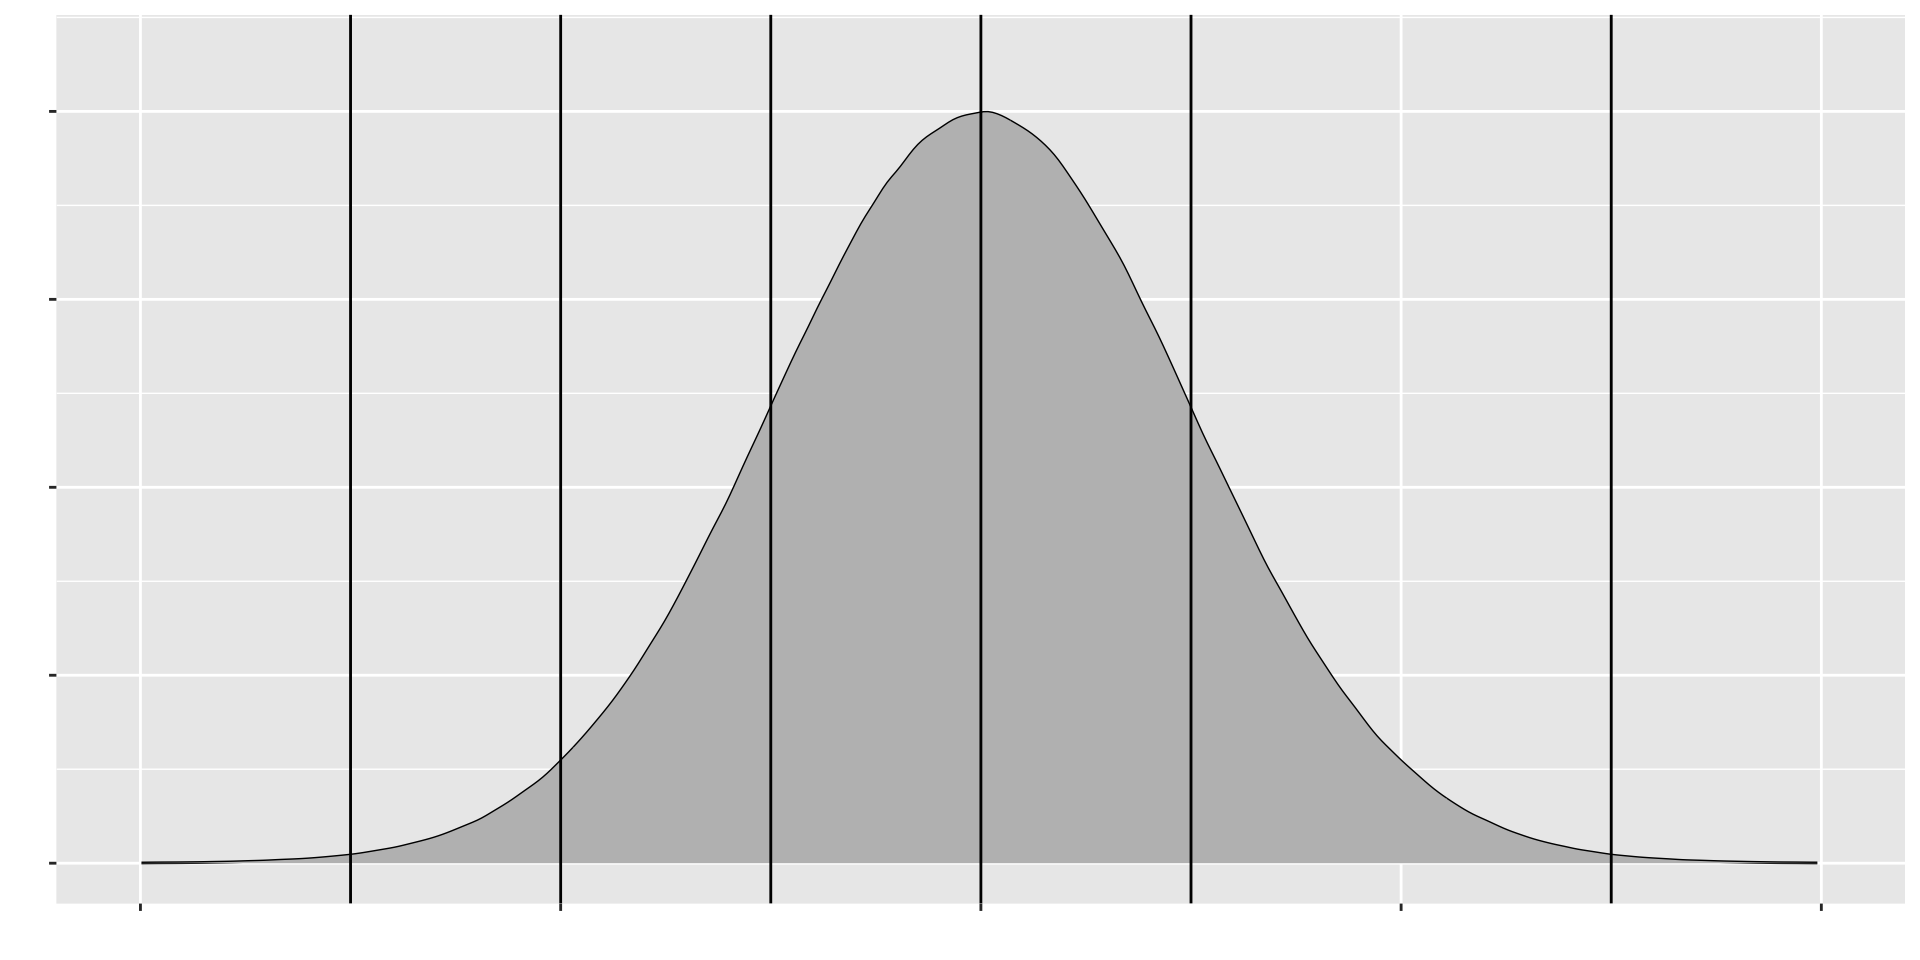
\includegraphics{figure/norm4-1} 

}

\caption{Empirical Rule for Normal Distribution}\label{fig:norm4}
\end{figure}

Calculate the following probabilities
1. \(P(|x-\mu|\leq \sigma)\)
2. \(P(|x-\mu|\leq 2\sigma)\)
3. \(P(|x-\mu|\leq 3\sigma)\)

\textbf{Empirical Rule for Normal Distribution}

Approximately 68\% of the values in any normal distribution lie within one standard deviation, approximately 95\% lie within two standard deviations and approximately 99.7\% lie within three standard deviations from the mean.

\begin{itemize}
\item
  The normal distribution is somewhat special as its two parameters \(\mu\) (the mean) and \(\sigma^2\) (the variance), provide us with complete information about the exact shape and location of the distribution.
\item
  Straightforward calculus shows that the normal distribution has its maximum at \(x=\mu\) and inflection point (where the curve changes from concave to convex) at \(\mu \pm\sigma.\)
\end{itemize}

\hypertarget{gamma-distribution}{%
\subsection{Gamma Distribution}\label{gamma-distribution}}

\begin{itemize}
\item
  We come across with many practical situations in which the variable of interest has a skewed distribution.
\item
  The gamma family of distributions is a flexible family of distributions on \([0,\infty)\) that yields a wide variety of skewed distributions
\end{itemize}

A random variable \(X\) is said to have a gamma distribution with shape parameter \(\alpha\) and scale parameter \(\beta\) if its probability density function is given by

\[f_X(x;\alpha, \beta)= \frac{1}{\Gamma(\alpha)\beta ^ {\alpha}}x^{\alpha-1}e^{-x/\beta}, \;\; 0<x<\infty,\;\; \alpha >0, \;\;\beta >0\]

Here \(\Gamma(\alpha)\) is called the \emph{gamma function},

\[\Gamma(\alpha)=\int_0^{\infty}x^{\alpha-1}e^{-x}dx\]
- The gamma function satisfies many useful relationships, in particular,

\begin{enumerate}
\def\labelenumi{\arabic{enumi}.}
\tightlist
\item
  \(\Gamma(\alpha+1)=\alpha\Gamma(\alpha),\;\; \alpha >0\) (can be verified through integration by parts)
\item
  \(\Gamma(1) =1\)
\item
  For any positive integer \(n(>0)\), \(\Gamma(n)=(n-1)!\)
\item
  \(\Gamma \left (\frac{1}{2} \right) = \sqrt{\pi}\)
\end{enumerate}

\begin{itemize}
\item
  When \(X\) has a gamma distribution with shape parameter \(\alpha\) and scale parameter \(\beta\), it is denoted as \(X \sim gamma(\alpha, \beta)\)
\item
  The parameter \(\alpha\) is known as the shape parameter, since it most influences the peakedness of the distibution
\item
  The parameter \(\beta\) is called the scale parameter, since most of its influence is on the spread of the distribution.
\end{itemize}

\begin{figure}

{\centering 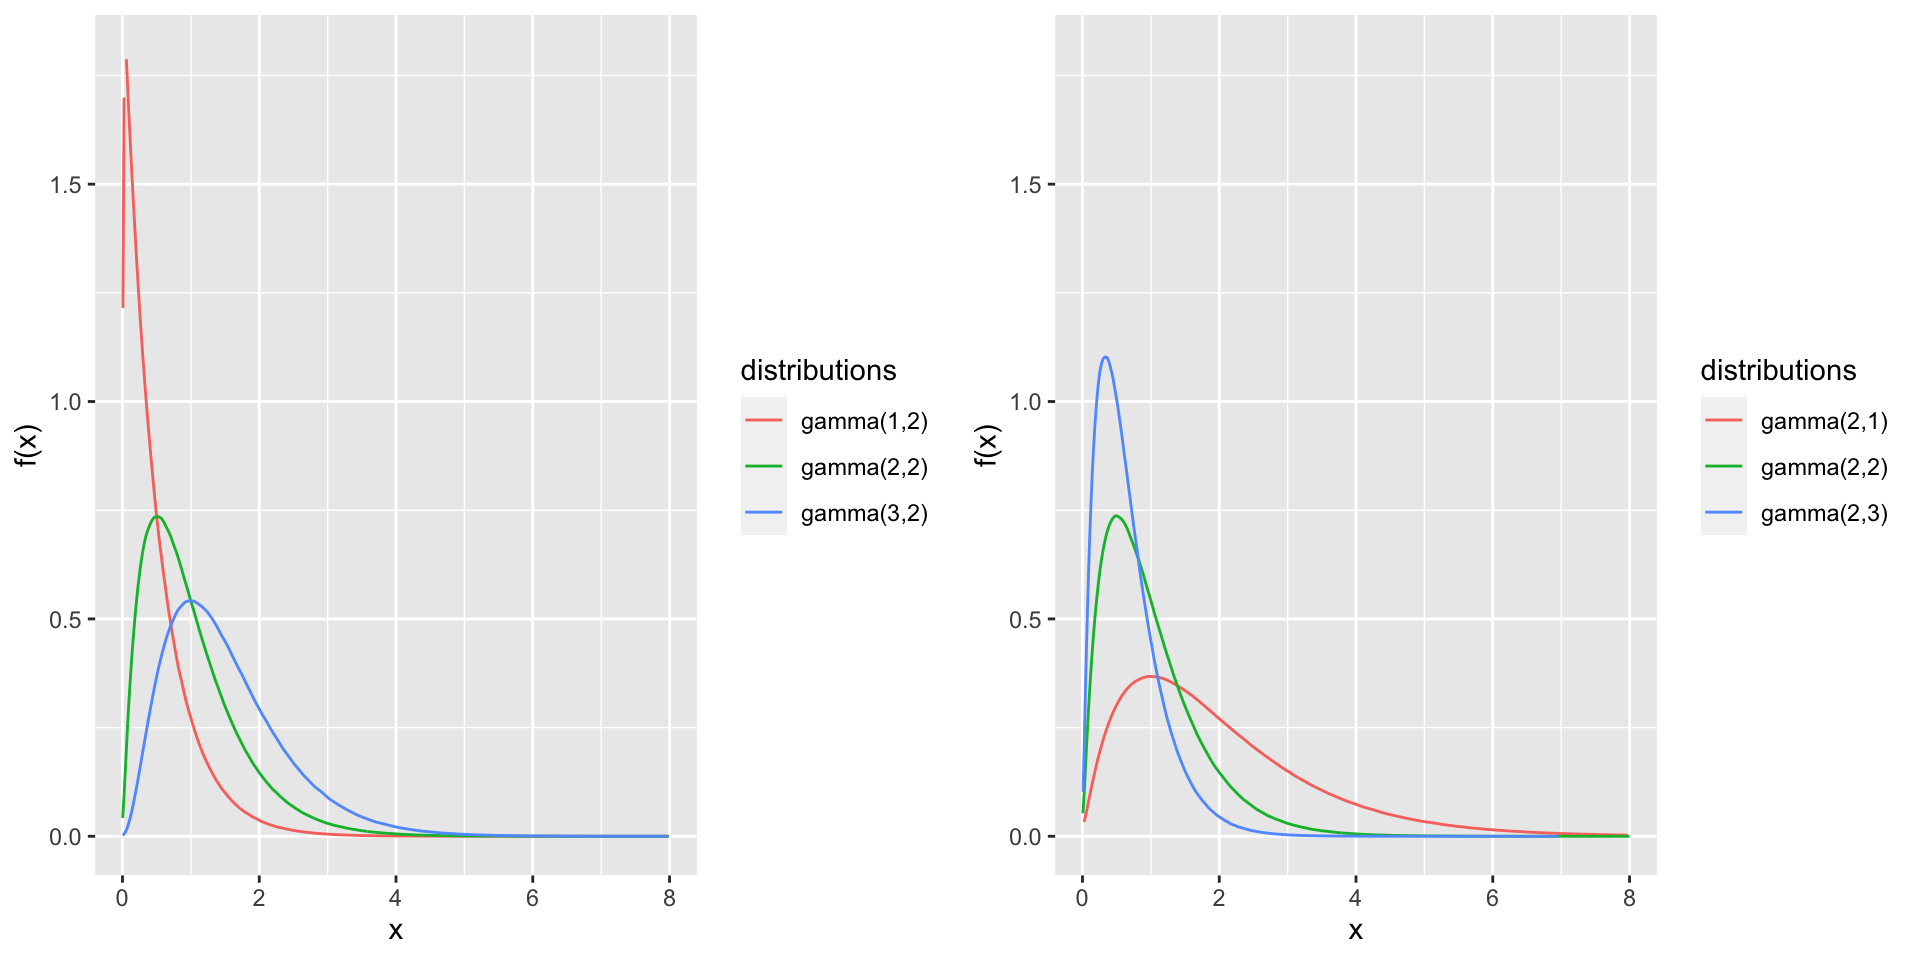
\includegraphics{figure/gamma-1} 

}

\caption{Gamma density functions}\label{fig:gamma}
\end{figure}

\begin{itemize}
\item
  If \(X\) has a gamma distribution with shape parameter \(\alpha\) and scale parameter \(\beta\), then

  \begin{itemize}
  \tightlist
  \item
    \(E(X) = \alpha \beta\)
  \item
    \(Var(X) = \alpha \beta^2\)
  \end{itemize}
\end{itemize}

\hypertarget{exponential-distribution}{%
\subsection{Exponential Distribution}\label{exponential-distribution}}

\begin{itemize}
\item
  This distribution is often used to model lifetime of various items.
\item
  When the number of events in a time interval has a Poisson distribution, the length of time interval between successive events can be modeled by an exponential distribution.
\item
  A random variable \(X\) is said to have an exponential distribution with scale parameter \(\beta\), if its probability density function is given by
\end{itemize}

\[f_X(x; \beta)=\frac{1}{\beta}e^{-x/\beta},\;\; 0<x<\infty\]

\begin{itemize}
\tightlist
\item
  This is denoted by \(X \sim exponential(\beta)\)
\end{itemize}

\begin{figure}

{\centering 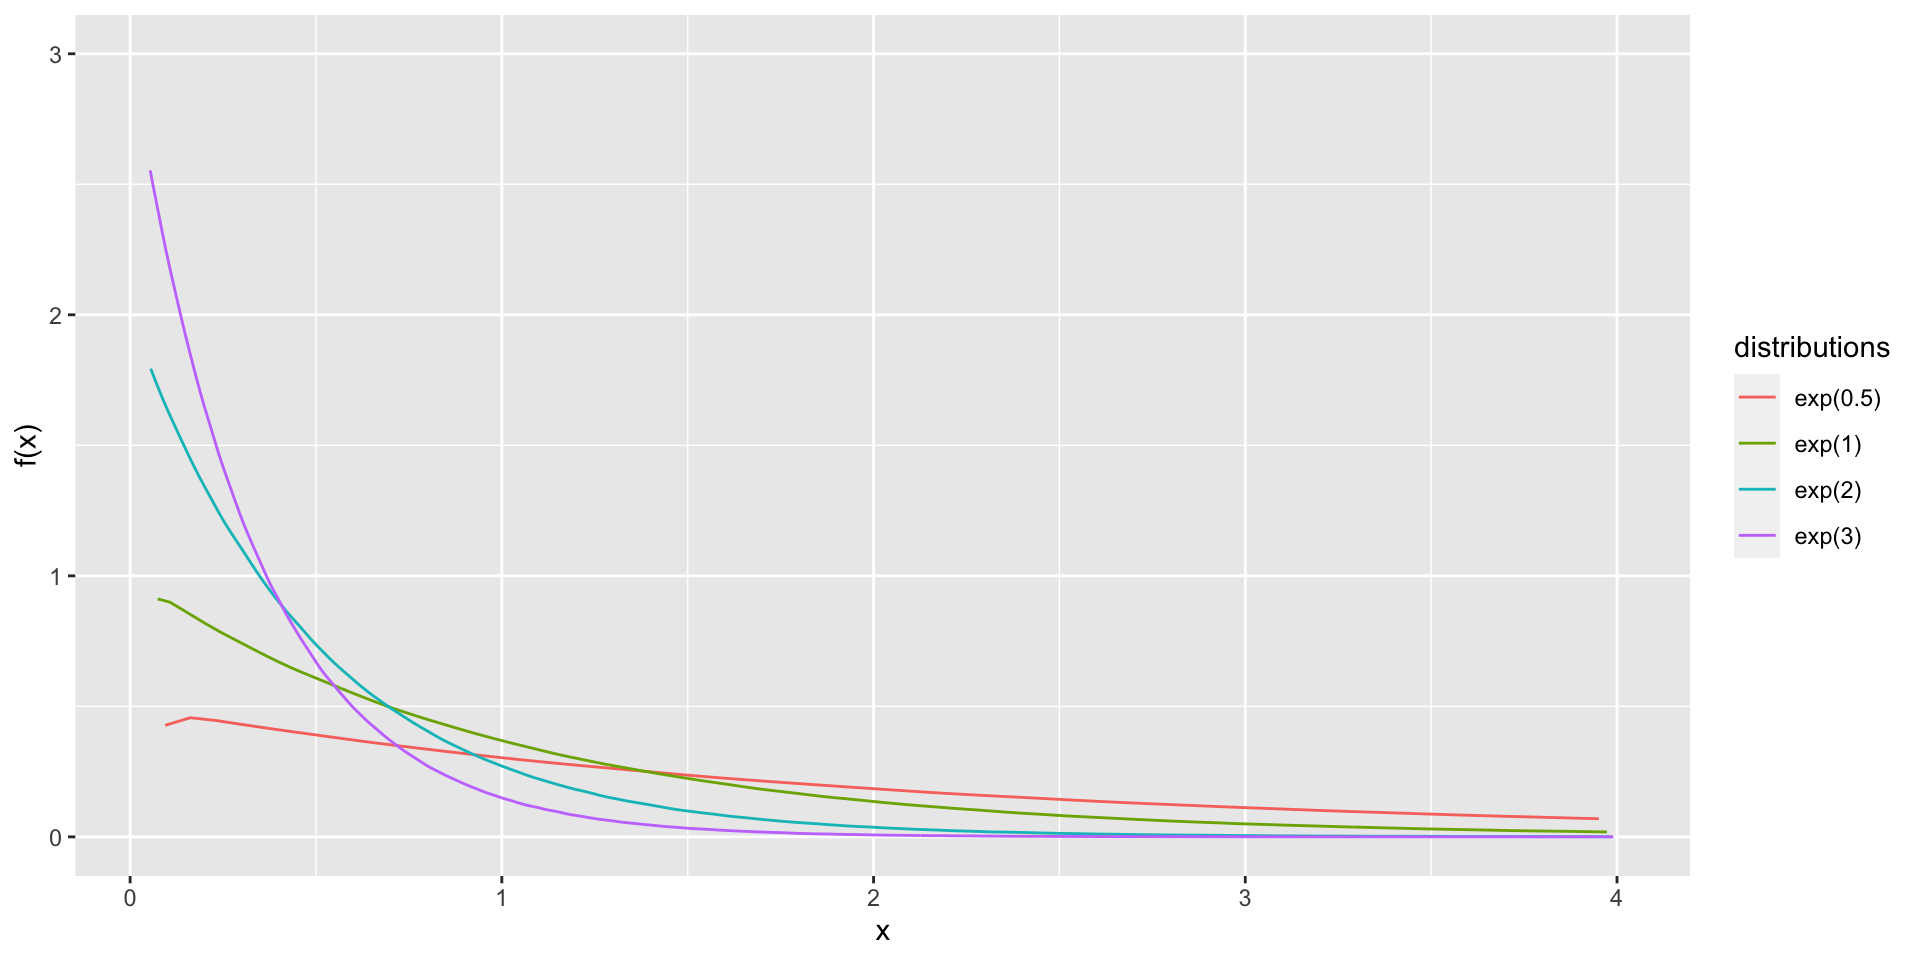
\includegraphics{figure/exp-1} 

}

\caption{Exponential density functions}\label{fig:exp}
\end{figure}

\begin{itemize}
\item
  Note that exponential distibution is a special case of the gamma distribution.
\item
  It can be easily shown that \(X\sim exponential(\beta) \iff X\sim gamma (1.\beta)\)
\item
  If \(X\) has an exponential distribution, then

  \begin{itemize}
  \tightlist
  \item
    \(E(X) = \beta\)
  \item
    \(Var(X) = \beta^{2}\)
  \end{itemize}
\end{itemize}

\hypertarget{beta-distribution}{%
\subsection{Beta Distribution}\label{beta-distribution}}

\begin{itemize}
\item
  The beta family of distributions is a continuous family on \((0,1)\) indexed by two parameters.
\item
  The \(beta(\alpha, \beta)\) probability density function is
\end{itemize}

\[f_X(x; \alpha, beta)= \frac{1}{B(\alpha, \beta)}x^{\alpha -1}(1-x)^{\beta-1},\;\;0<x<1,\; \alpha >0,\;\; \beta >0,\]

where \(B(\alpha, \beta)\) denotes the \emph{beta function},
\[B(\alpha, \beta)=\int_0^1x^{\alpha -1}(1-x)^{\beta-1}dx.\]

\begin{itemize}
\item
  The beta function is related to the gamma function through the following identity \[B(\alpha, \beta)= \frac{\Gamma(\alpha)\Gamma(\beta)}{\Gamma(\alpha+\beta)}\]
\item
  The beta distibution is one of the few common ``named'' distributions that give probability 1 to a finite interval, here taken to be \((0,1)\).
\item
  Therefore, the beta distibution is often used to model proportions, which naturally lie between 0 and 1.
\end{itemize}

\begin{figure}

{\centering 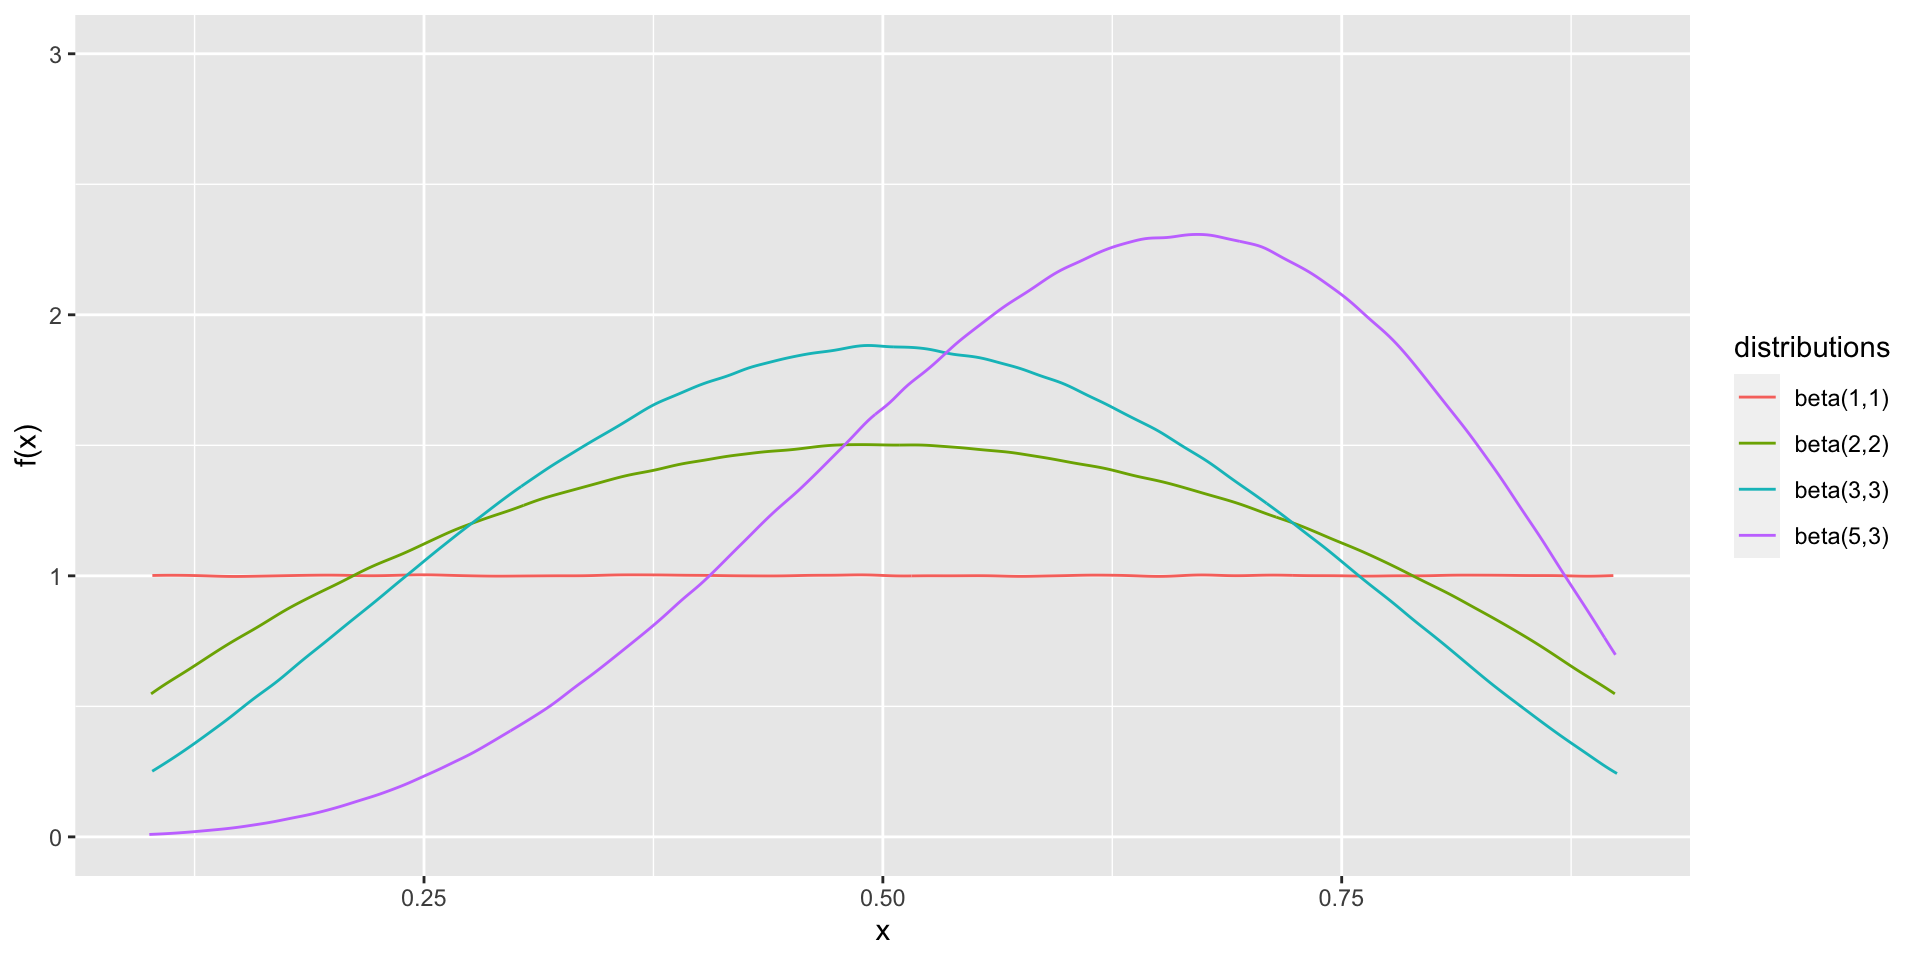
\includegraphics{figure/beta-1} 

}

\caption{Beta density functions}\label{fig:beta}
\end{figure}
\newpage

\hypertarget{approximations}{%
\section{Approximations}\label{approximations}}

\hypertarget{poisson-approximation-to-binomial}{%
\subsection{Poisson approximation to Binomial}\label{poisson-approximation-to-binomial}}

Suppose \(X\sim Bin(n, \theta)\) and \(n\) is large and \(\theta\) is small. Then \(X\sim Poisson(n\theta)\) and

\[f_X(x) \approx \frac{e^{-n\theta} (n\theta)^x}{x!}\]

\emph{Example 16}

Suppose \(X\) has a binomial distribution with \(n=40\) and \(p=0.005\). Find \(f_X(1)\)

\hypertarget{normal-approximation-to-binomial}{%
\subsection{Normal approximation to Binomial}\label{normal-approximation-to-binomial}}

Suppose \(X\sim Bin(n, \theta)\) and \(n\theta \geq 5\) and \(n(1-\theta) \geq 5.\) Then \(X \sim N(n\theta, n\theta(1-\theta))\) and

\[P(X \leq x)_{Binomial} = P(X \leq x + 0.5)_{Normal} \approx P(Z \leq \frac{x+0.5-n\theta}{\sqrt{n\theta(1-\theta)}})\]

\textbf{Note:} Since we are approximating a discrete distribution by a continuous distribution, we should apply a \emph{continuity correction}

\emph{Example 17}

Suppose \(X\) has a binomial distribution with \(n=40\) and \(p=0.6.\) Find

\begin{enumerate}
\def\labelenumi{\arabic{enumi}.}
\tightlist
\item
  \(P(X\leq 20)\)
\item
  \(P(X < 25)\)
\item
  \(P(X > 15)\)
\item
  \(P(X \geq 20)\)
\item
  \(P(X = 30)\)
\end{enumerate}

\hypertarget{normal-approximation-to-poisson}{%
\subsection{Normal approximation to Poisson}\label{normal-approximation-to-poisson}}

Suppose \(X\sim Poisson(\lambda)\) and \(\lambda > 10,\)

\[P(X \leq x)_{Poisson} = P(X \leq x + 0.5)_{Normal} \approx P(Z \leq \frac{x+0.5-\lambda}{\sqrt{\lambda}})\]

\textbf{Note:} Since we are approximating a discrete distribution by a continuous distribution, we should apply a \emph{continuity correction}

\emph{Example 18}

Suppose \(X\) has a Poisson distribution with \(\lambda=25\)

\begin{enumerate}
\def\labelenumi{\arabic{enumi}.}
\tightlist
\item
  \(P(X\leq 20)\)
\item
  \(P(X < 25)\)
\item
  \(P(X > 15)\)
\item
  \(P(X \geq 20)\)
\item
  \(P(X = 30)\)
\end{enumerate}

\hypertarget{distribution-of-functions-of-random-variables}{%
\section{Distribution of Functions of Random Variables}\label{distribution-of-functions-of-random-variables}}

\begin{enumerate}
\def\labelenumi{\arabic{enumi}.}
\tightlist
\item
  \textbf{Distribution of the linear transformation of a normal random variable}
\end{enumerate}

Suppose that \(X \sim N(\mu, \sigma^2).\) Let \(Y= ax+b,\) where \(a\) and \(b\) are constants. Then

\[Y\sim N(a\mu +b, a^2\sigma^2)\]

\begin{enumerate}
\def\labelenumi{\arabic{enumi}.}
\setcounter{enumi}{1}
\tightlist
\item
  \textbf{Standardization of a normal random variable}
\end{enumerate}

Suppose that \(X \sim N(\mu, \sigma^2).\) Let \(Z= \frac{X-\mu}{\sigma}.\) Then

\[Z\sim N(0,1).\]

\begin{enumerate}
\def\labelenumi{\arabic{enumi}.}
\setcounter{enumi}{2}
\tightlist
\item
  \textbf{Distribution of the square of a standard normal random variable}
\end{enumerate}

Suppose that \(Z \sim N(0,1).\) Let \(Y= Z^2.\) Then

\[Y\sim \chi^2_1\]

\newpage

\hypertarget{distribution-of-sum-of-independent-random-variables}{%
\section{Distribution of Sum of Independent Random Variables}\label{distribution-of-sum-of-independent-random-variables}}

\begin{enumerate}
\def\labelenumi{\arabic{enumi}.}
\tightlist
\item
  \textbf{Distribution of sum of i.i.d Bernoulli random variables}
\end{enumerate}

Suppose that \(X_1, X_2, \dots, X_n\) are independent, identically distributed (i.i.d) random variables with \(Bernoulli(\theta)\) distribution. Let \(Y= X_1+X_2+\dots +X_n.\) Then

\[Y\sim Bin(n, \theta); \;\;y=0,1,2,\dots, n.\]

\begin{enumerate}
\def\labelenumi{\arabic{enumi}.}
\setcounter{enumi}{1}
\tightlist
\item
  \textbf{Distribution of sum of i.i.d Poisson random variables}
\end{enumerate}

Suppose that \(X_1, X_2, \dots, X_n\) are independent, identically distributed (i.i.d) random variables with \(Poisson(\lambda)\) distribution. Let \(Y= X_1+X_2+\dots +X_n.\) Then

\[Y\sim Poisson(n\lambda); \;\;y=0,1,2,\dots,.\]

\begin{enumerate}
\def\labelenumi{\arabic{enumi}.}
\setcounter{enumi}{2}
\tightlist
\item
  \textbf{Distribution of sum of independent Poisson random variables}
\end{enumerate}

Suppose that \(X_1, X_2, \dots, X_n\) are independent random variables with \(Poisson(\lambda_i), \; i=1,2,\dots, n.\) Let \(Y= X_1+X_2+\dots +X_n.\) Then

\[Y\sim Poisson \left(\sum_{i=1}^n\lambda_i\right); \;\;y=0,1,2,\dots,.\]

\begin{enumerate}
\def\labelenumi{\arabic{enumi}.}
\setcounter{enumi}{3}
\tightlist
\item
  \textbf{Distribution of sum of i.i.d Geometric random variables}
\end{enumerate}

Suppose that \(X_1, X_2, \dots, X_n\) are independent, identically distributed (i.i.d) random variables with \(Geometric(\theta)\) distribution. Let \(Y= X_1+X_2+\dots +X_n.\) Then

\[Y\sim Neg.bin(n, \theta); \;\;y=n, n+1, n+2,\dots,.\]

\begin{enumerate}
\def\labelenumi{\arabic{enumi}.}
\setcounter{enumi}{4}
\tightlist
\item
  \textbf{Distribution of sum of independent Normal random variables}
\end{enumerate}

Suppose that \(X_1, X_2, \dots, X_n\) are independent random variables with \(X_i\sim N(\mu_i, \sigma_i^2); \; i=1,2,\dots, n\). Let \(Y= X_1+X_2+\dots +X_n.\) Then

\[Y\sim N\left(\sum_{i=1}^n \mu_i,\sum_{i=1}^n \sigma_i^2  \right).\]

\begin{enumerate}
\def\labelenumi{\arabic{enumi}.}
\setcounter{enumi}{5}
\tightlist
\item
  \textbf{Distribution of sum of i.i.d exponential random variables}
\end{enumerate}

Suppose that \(X_1, X_2, \dots, X_n\) are independent, identically distributed (i.i.d) random variables with \(X_i\sim exp(\lambda);\; i=1,2,\dots, n\). Let \(Y= X_1+X_2+\dots +X_n.\) Then

\[Y \sim gamma(n, \lambda)\]

\begin{enumerate}
\def\labelenumi{\arabic{enumi}.}
\setcounter{enumi}{6}
\tightlist
\item
  \textbf{Distribution of sum of independent gamma random variables}
\end{enumerate}

Suppose that \(X_1, X_2, \dots, X_n\) are independent random variables with \(X_i\sim gamma(\alpha_i, \lambda);\; i=1,2,\dots, n\). Let \(Y= X_1+X_2+\dots +X_n.\) Then

\[Y \sim gamma\left(\sum_{i=1}^n\alpha_i, \lambda\right).\]

\hypertarget{sampling-distribution}{%
\section{Sampling Distribution}\label{sampling-distribution}}

\begin{enumerate}
\def\labelenumi{\arabic{enumi}.}
\tightlist
\item
  \textbf{Distribution of sample mean of a normal distribution}
\end{enumerate}

Suppose that \(X_1, X_2, \dots, X_n\) is a random sample from a normal distribution with mean \(\mu\) and variance \(\sigma^2\). Let \(\bar{X} = \frac{X_1+X_2+\dots + X_n}{n}\) be the sample mean. Then,

\[\bar{X} \sim N\left(\mu, \frac{\sigma^2}{n}\right)\]

\begin{enumerate}
\def\labelenumi{\arabic{enumi}.}
\setcounter{enumi}{1}
\tightlist
\item
  \textbf{Distribution of sample variance of a normal distribution}
\end{enumerate}

Suppose that \(X_1, X_2, \dots, X_n\) is a random sample from a normal distribution with mean \(\mu\) and variance \(\sigma^2\). Let \(\bar{X} = \frac{X_1+X_2+\dots + X_n}{n}\) be the sample mean and \(S^2 = \frac{1}{n-1}\sum_{i=1}^n(X_i-\bar{X})^2\) be the sample variance. Then,

\[\frac{(n-1)S^2}{\sigma^2} \sim \chi^2_{n-1}.\]

\begin{enumerate}
\def\labelenumi{\arabic{enumi}.}
\setcounter{enumi}{2}
\tightlist
\item
  \textbf{Large sample distribution of sample average - Central Limit Theorem)}
\end{enumerate}

Suppose that \(X_1, X_2, \dots, X_n\) is a random sample from any distribution with mean \(\mu\) and variance \(\sigma^2\). Let \(\bar{X} = \frac{X_1+X_2+\dots + X_n}{n}\) be the sample mean and \(Z_n = \frac{\bar{X}_n-\mu}{\sigma/\sqrt{n}}.\)

Then, the distribution of \(Z_n\) approaches the standard normal distribution as \(n\) approaches \(\infty.\)

\hypertarget{references}{%
\section*{References}\label{references}}
\addcontentsline{toc}{section}{References}

Casella, G., \& Berger, R. L. (2002). Statistical inference (Vol. 2, pp.~337-472).Pacific Grove, CA: Duxbury

Mood, A.M., Graybill, F.A. and Boes, D.C. (2007): Introduction to the Theory of Statistics, 3rd Edn. (Reprint). Tata McGraw-Hill Pub. Co.~Ltd.

\newpage
\pagenumbering{arabic}

\hypertarget{tutorial}{%
\section*{Tutorial}\label{tutorial}}
\addcontentsline{toc}{section}{Tutorial}

\begin{enumerate}
\def\labelenumi{\arabic{enumi}.}
\tightlist
\item
  Consider the experiment of taking two products randomly form a production line and determine whether each is defective or not. Express the following events using a suitably defined random variable.
\end{enumerate}

\(D_0=\) \emph{The event that both products are non defective}

\(D_1=\) \emph{The event that one product is defective}

\(D_2=\) \emph{The event that both products are defective}

\(E=\) \emph{The event that at least one product is defective}

\begin{enumerate}
\def\labelenumi{\arabic{enumi}.}
\setcounter{enumi}{1}
\tightlist
\item
  Let X be a random variable with the following probability distribution
\end{enumerate}

\begin{longtable}[]{@{}lllllll@{}}
\toprule
\(x\) & 1 & 1.5 & 2 & 2.5 & 3 & other\tabularnewline
\midrule
\endhead
\(f_X(x)\) & \(k\) & \(2k\) & \(4k\) & \(2k\) & \(k\) & 0\tabularnewline
\bottomrule
\end{longtable}

\begin{enumerate}
\def\labelenumi{(\alph{enumi})}
\tightlist
\item
  Find the value of \(k\)
\item
  Find \(P(X = 2.5)\)
\item
  Calculate \(P (X \geq 1.75)\)
\end{enumerate}

\begin{enumerate}
\def\labelenumi{\arabic{enumi}.}
\setcounter{enumi}{2}
\tightlist
\item
  The sample space of a random experiment is \(\{a, b, c, d, e, f\}\), and each outcome is equally likely. A random variable \(X\) is defined as follows:
\end{enumerate}

\begin{longtable}[]{@{}lllllll@{}}
\toprule
Outcome & \(a\) & \(b\) & \(c\) & \(d\) & \(e\) & \(f\)\tabularnewline
\midrule
\endhead
\(x\) & 0 & 0 & 1.5 & 1.5 & 2 & 3\tabularnewline
\bottomrule
\end{longtable}

Determine the probability mass function of \(X\). Use the probability mass function to determine the following probabilities:

\begin{enumerate}
\def\labelenumi{(\alph{enumi})}
\tightlist
\item
  \(P(X = 1.5)\)
\item
  \(P(0.5 < X < 2.7)\)
\item
  \(P(X > 3)\)
\item
  \(P(0 \leq X < 2)\)
\item
  \(P(X = 0 \text{ or } X = 2)\)
\end{enumerate}

\begin{enumerate}
\def\labelenumi{\arabic{enumi}.}
\setcounter{enumi}{3}
\tightlist
\item
  Verify that the following function is a probability mass function, and determine the requested probabilities.
\end{enumerate}

\[f_X(x)=\frac{8}{7} \left(\frac{1}{2} \right)^x, \text{ x= 1,2,3 }\]

\begin{enumerate}
\def\labelenumi{(\alph{enumi})}
\tightlist
\item
  \(P(X \leq 1)\)
\item
  \(P(X > 1)\)
\item
  \(P (2 < X < 6)\)
\item
  \(P(X \leq 1 \text{ or } X > 1)\)
\end{enumerate}

\begin{enumerate}
\def\labelenumi{\arabic{enumi}.}
\setcounter{enumi}{4}
\tightlist
\item
  A disk drive manufacturer sells storage devices with capacities of one terabyte, 500 gigabytes, and 100 gigabytes with probabilities 0.5, 0.3, and 0.2, respectively. The revenues associated with the sales in that year are estimated to be \$50 million, \$25 million, and \$10 million, respectively. Let \(X\) denotes the revenue of storage devices during that year.
\end{enumerate}

\begin{enumerate}
\def\labelenumi{(\alph{enumi})}
\tightlist
\item
  Determine the probability mass function of \(X\).
\item
  Calculate the probability of getting more than \$20 million of revenue during that year.\\
\item
  Determine the cumulative distribution function of \(X\)
\end{enumerate}

\begin{enumerate}
\def\labelenumi{\arabic{enumi}.}
\setcounter{enumi}{5}
\tightlist
\item
  Consider the following cumulative distribution function:
\end{enumerate}

\begin{equation}
F_X(x) =
\begin{cases} 
0 & x<-2\\
0.2 & -2 \leq x< 0\\
0.7 & 0\leq x<2\\
1 & 2 \leq x
\end{cases}
\end{equation}

\begin{enumerate}
\def\labelenumi{\alph{enumi})}
\tightlist
\item
  Draw the plot of \(F_X(x)\)
\item
  Discuss the properties of \(F_X(x)\) (eg: whether it is discrete or continuous, whether it is decreasing or increasing function etc. )
\item
  Determine the probability mass function of \(X\) from the above cumulative distribution function:
\item
  Plot the probability mass function of \(X\)
\end{enumerate}

\begin{enumerate}
\def\labelenumi{\arabic{enumi}.}
\setcounter{enumi}{6}
\tightlist
\item
  The number of e-mail messages received per hour varies from 10 to 16 with the following probabilities
\end{enumerate}

\begin{longtable}[]{@{}llllllll@{}}
\toprule
\(x =\) number of messages & 10 & 11 & 12 & 13 & 14 & 15 & 16\tabularnewline
\midrule
\endhead
\(P(X=x)\) & 0.08 & 0.15 & 0.1 & 0.2 & 0.1 & 0.07 & 0.3\tabularnewline
\bottomrule
\end{longtable}

\begin{enumerate}
\def\labelenumi{\alph{enumi})}
\tightlist
\item
  Let \(X\) be the number of e-mail messages received per hour. Find the probability mass function of X
\item
  Determine the mean and standard deviation of the number of messages received per hour
\end{enumerate}

\begin{enumerate}
\def\labelenumi{\arabic{enumi}.}
\setcounter{enumi}{7}
\tightlist
\item
  According to past data, twenty percent of all telephones of a certain type are submitted for service while under warranty. Of these, \(60\%\) can be repaired whereas the other \(40\%\) must be replaced with new units. If a company purchases ten of these telephones, what is the probability that
\end{enumerate}

\begin{enumerate}
\def\labelenumi{\alph{enumi})}
\tightlist
\item
  two telephones will be submitted for service under warranty?
\item
  at most 3 telephones will be submitted for service under warranty?
\item
  two telephones will end up being replaced under warranty?
\item
  one telephone will end up being repaired under warranty?
\end{enumerate}

\begin{enumerate}
\def\labelenumi{\arabic{enumi}.}
\setcounter{enumi}{8}
\tightlist
\item
  Each sample of water has a \(10\%\) chance of containing a particular organic pollutant. Assume that the samples are independent with regard to the presence of the pollutant. Find the probability that in the next 18 samples, exactly 2 contain the pollutant
\end{enumerate}

\begin{enumerate}
\def\labelenumi{\alph{enumi})}
\tightlist
\item
  Define a suitable random variable for the above question
\item
  Find the distribution of that random variable
\item
  Find the probability that in the next 18 samples, exactly 2 contain the pollutant
\end{enumerate}

\begin{enumerate}
\def\labelenumi{\arabic{enumi}.}
\setcounter{enumi}{9}
\tightlist
\item
  The space shuttle flight control system called Primary Avionics Software Set (PASS) uses four independent computers working in parallel. At each critical step, the computers ``vote'' to determine the appropriate step. The probability that a computer will ask for a roll to the left when a roll to the right is appropriate is 0.0001. Let \(X\) denotes the number of computers that vote for a left roll when a right roll is appropriate.
\end{enumerate}

\begin{enumerate}
\def\labelenumi{\alph{enumi})}
\tightlist
\item
  What is the probability mass function of \(X\)?
\item
  What are the mean and variance of \(X\)?
\end{enumerate}

\begin{enumerate}
\def\labelenumi{\arabic{enumi}.}
\setcounter{enumi}{10}
\tightlist
\item
  A University lecturer never finishes his lecture before the end of the hour and always finishes his lectures within 2 minutes after the hour. Let \(X\) = the time that elapses between the end of the hour and the end of the lecture and suppose the pdf of \(X\) is
\end{enumerate}

\begin{equation}
f_X(x) =
\begin{cases} 
kx^2 & 0\leq  x\leq 2\\
0 & otherwise
\end{cases}
\end{equation}

\begin{enumerate}
\def\labelenumi{\alph{enumi})}
\tightlist
\item
  Find the value of \(k\) and draw the density curve.
\item
  What is the probability that the lecture ends within 1 min of the end of the hour?
\item
  What is the probability that the lecture continues beyond the hour for between 60 and 90 sec?
\item
  What is the probability that the lecture continues for at least 90 sec beyond the end of the hour?
\end{enumerate}

\begin{enumerate}
\def\labelenumi{\arabic{enumi}.}
\setcounter{enumi}{11}
\tightlist
\item
  The daily sales of gasoline are uniformly distributed between 2,000 and 5,000 gallons. Find the probability that sales are:
\end{enumerate}

\begin{enumerate}
\def\labelenumi{\alph{enumi})}
\tightlist
\item
  between 2,500 and 3,000 gallon
\item
  more than 4000 gallons
\item
  exactly 2500 gallons
\end{enumerate}

\begin{enumerate}
\def\labelenumi{\arabic{enumi}.}
\setcounter{enumi}{12}
\tightlist
\item
  Suppose \(X\) has a continuous uniform distribution over the interval \([-1,1]\). Determine the following:
\end{enumerate}

\begin{enumerate}
\def\labelenumi{(\alph{enumi})}
\tightlist
\item
  Mean, variance, and standard deviation of \(X\)
\item
  Value for \(k\) such that \(P(-k < X < k ) = 0.90\)
\item
  Cumulative distribution function
\end{enumerate}

\begin{enumerate}
\def\labelenumi{\arabic{enumi}.}
\setcounter{enumi}{13}
\tightlist
\item
  Suppose that the time it takes a data collection operator to fill out an electronic form for a database is uniformly between 1.5 and 2.2 minutes.
\end{enumerate}

\begin{enumerate}
\def\labelenumi{\alph{enumi})}
\tightlist
\item
  What are the mean and variance of the time it takes an operator to fill out the form?
\item
  What is the probability that it will take less than two minutes to fill out the form?
\item
  Determine the cumulative distribution function of the time it takes to fill out the form.
\end{enumerate}

\begin{enumerate}
\def\labelenumi{\arabic{enumi}.}
\setcounter{enumi}{14}
\item
  An electronic product contains 40 integrated circuits. The probability that any integrated circuit is defective is 0.01, and the integrated circuits are independent. The product operates only if there are no defective integrated circuits. What is the probability that the product operates?
\item
  A bag of 200 chocolate chips is dumped into a batch of cookies dough. 40 cookies are made from such a batch of dough. What is the probability that a randomly selected cookie has at least 4 chocolate chips?
\item
  For the case of the thin copper wire, suppose that the number of flaws follows a Poisson distribution with a mean of 2.3 flaws per millimeter.
\end{enumerate}

\begin{enumerate}
\def\labelenumi{\alph{enumi})}
\item
  Determine the probability of exactly two flaws in 1 millimeter of wire.
\item
  Determine the probability of 10 flaws in 5 millimeters of wire
\end{enumerate}

\begin{enumerate}
\def\labelenumi{\arabic{enumi}.}
\setcounter{enumi}{17}
\tightlist
\item
  Contamination is a problem in the manufacture of magnetic storage disks. Assume that the number of particles of contamination that occur on a disk surface has a Poisson distribution, and the average number of particles per square centimeter of media surface is 0.1. The area of a disk under study is 100 square centimeters.
\end{enumerate}

\begin{enumerate}
\def\labelenumi{\alph{enumi})}
\item
  Determine the probability that 12 particles occur in the area of a disk under study.
\item
  Determine the probability that zero particles occur in the area of the disk under study.
\item
  Determine the probability that 12 or fewer particles occur in the area of the disk under study
\end{enumerate}

\begin{enumerate}
\def\labelenumi{\arabic{enumi}.}
\setcounter{enumi}{18}
\tightlist
\item
  The number of surface flaws in plastic panels used in the interior of automobiles has a Poisson distribution with a mean of 0.05 flaw per square foot of plastic panel. Assume that an automobile interior contains 10 square feet of plastic panel.
\end{enumerate}

\begin{enumerate}
\def\labelenumi{\alph{enumi})}
\item
  What is the probability that there are no surface flaws in an auto's interior?
\item
  If 10 cars are sold to a rental company, what is the probability that none of the 10 cars has any surface flaws?
\item
  If 10 cars are sold to a rental company, what is the probability that at most 1 car has any surface flaws?
\end{enumerate}

\begin{enumerate}
\def\labelenumi{\arabic{enumi}.}
\setcounter{enumi}{19}
\tightlist
\item
  Cabs pass your workplace according to a Poisson process with a mean of five cabs per hour. Suppose that you exit the workplace at 6:00 p.m. Determine the following:
\end{enumerate}

\begin{enumerate}
\def\labelenumi{\alph{enumi})}
\item
  Probability that you wait more than 10 minutes for a cab.
\item
  Probability that you wait fewer than 20 minutes for a cab.
\end{enumerate}

\newpage

\begin{enumerate}
\def\labelenumi{\arabic{enumi}.}
\setcounter{enumi}{10}
\tightlist
\item
  An electronic product contains 40 integrated circuits. The probability that any integrated circuit is defective is 0.01, and the integrated circuits are independent. The product operates only if there are no defective integrated circuits. What is the probability that the product operates?
\end{enumerate}

\begin{enumerate}
\def\labelenumi{\arabic{enumi}.}
\setcounter{enumi}{6}
\tightlist
\item
  A person must take two buses to go to work. From the past experience, he knows that a bus can come at any time within 6 minutes. Also, the probability that a bus comes within any period of the same length is the same. Hence, it is reasonable to assume the following probability density function for the waiting time \(X\) (in minutes) for a bus
\end{enumerate}

\(f_X(x) = \frac{1}{6}, \;\;0<x<6.\)

Then the total waiting time \(T\) at both bus-stops has the following density function

\begin{equation}
f_T(t) =
\begin{cases} 
\frac{t}{36} & 0\leq t \leq 6\\
\frac{1}{3}- \frac{t}{36} & 6\leq t \leq 12
\end{cases}
\end{equation}

\begin{enumerate}
\def\labelenumi{\alph{enumi})}
\tightlist
\item
  Verify that each of above function is a proper density function
\item
  What is the probability that the waiting time at the first bus-stop will be less than 2 minutes?
\item
  What is the probability that the waiting time at the first bus-stop will be less than 2 minutes and the waiting time at the second
\end{enumerate}

\newpage
\pagenumbering{arabic}
\begin{landscape}

\hypertarget{summary}{%
\section*{Summary}\label{summary}}
\addcontentsline{toc}{section}{Summary}

\textbf{Models for Discrete Distributions}

\begin{longtable}[]{@{}lllllll@{}}
\toprule
\begin{minipage}[b]{0.10\columnwidth}\raggedright
Name\strut
\end{minipage} & \begin{minipage}[b]{0.13\columnwidth}\raggedright
Remarks\strut
\end{minipage} & \begin{minipage}[b]{0.16\columnwidth}\raggedright
Probability mass function\strut
\end{minipage} & \begin{minipage}[b]{0.14\columnwidth}\raggedright
values of \(X\)\strut
\end{minipage} & \begin{minipage}[b]{0.16\columnwidth}\raggedright
Parameter Space\strut
\end{minipage} & \begin{minipage}[b]{0.05\columnwidth}\raggedright
Mean\strut
\end{minipage} & \begin{minipage}[b]{0.09\columnwidth}\raggedright
Variance\strut
\end{minipage}\tabularnewline
\midrule
\endhead
\begin{minipage}[t]{0.10\columnwidth}\raggedright
Discrete Uniform\strut
\end{minipage} & \begin{minipage}[t]{0.13\columnwidth}\raggedright
Outcomes that are equally likely (finite)\strut
\end{minipage} & \begin{minipage}[t]{0.16\columnwidth}\raggedright
\(f(x) = \frac{1}{N}\)\strut
\end{minipage} & \begin{minipage}[t]{0.14\columnwidth}\raggedright
\(x=1,2,\dots, N\)\strut
\end{minipage} & \begin{minipage}[t]{0.16\columnwidth}\raggedright
\(N=1,2,\dots\)\strut
\end{minipage} & \begin{minipage}[t]{0.05\columnwidth}\raggedright
\(\frac{N+1}{2}\)\strut
\end{minipage} & \begin{minipage}[t]{0.09\columnwidth}\raggedright
\(\frac{N^2-1}{12}\)\strut
\end{minipage}\tabularnewline
\begin{minipage}[t]{0.10\columnwidth}\raggedright
Bernoulli\strut
\end{minipage} & \begin{minipage}[t]{0.13\columnwidth}\raggedright
Bernoulli trial\strut
\end{minipage} & \begin{minipage}[t]{0.16\columnwidth}\raggedright
\(f(x) = \theta^x (1-\theta)^{1-x}\)\strut
\end{minipage} & \begin{minipage}[t]{0.14\columnwidth}\raggedright
\(x=0,1\)\strut
\end{minipage} & \begin{minipage}[t]{0.16\columnwidth}\raggedright
\(0\leq \theta \leq 1\)\strut
\end{minipage} & \begin{minipage}[t]{0.05\columnwidth}\raggedright
\(\theta\)\strut
\end{minipage} & \begin{minipage}[t]{0.09\columnwidth}\raggedright
\(\theta (1-\theta)\)\strut
\end{minipage}\tabularnewline
\begin{minipage}[t]{0.10\columnwidth}\raggedright
Binomial\strut
\end{minipage} & \begin{minipage}[t]{0.13\columnwidth}\raggedright
\(X=\) Number of successes in \(n\) fixed trials\strut
\end{minipage} & \begin{minipage}[t]{0.16\columnwidth}\raggedright
\(f_X(x) = {n\choose x}\theta ^x(1-\theta)^{n-x}\)\strut
\end{minipage} & \begin{minipage}[t]{0.14\columnwidth}\raggedright
\(x=0,1,2,\dots, n\)\strut
\end{minipage} & \begin{minipage}[t]{0.16\columnwidth}\raggedright
\(0\leq \theta \leq 1; \;\;\; \newline n =1,2,3,\dots\)\strut
\end{minipage} & \begin{minipage}[t]{0.05\columnwidth}\raggedright
\(n\theta\)\strut
\end{minipage} & \begin{minipage}[t]{0.09\columnwidth}\raggedright
\(n\theta(1-\theta)\)\strut
\end{minipage}\tabularnewline
\begin{minipage}[t]{0.10\columnwidth}\raggedright
Geometric\strut
\end{minipage} & \begin{minipage}[t]{0.13\columnwidth}\raggedright
\(X=\) Number of failures before the first success\strut
\end{minipage} & \begin{minipage}[t]{0.16\columnwidth}\raggedright
\(f_X(x)= \theta (1-\theta)^x\)\strut
\end{minipage} & \begin{minipage}[t]{0.14\columnwidth}\raggedright
\(x=0,1,2,\dots\)\strut
\end{minipage} & \begin{minipage}[t]{0.16\columnwidth}\raggedright
\(0\leq \theta \leq 1\)\strut
\end{minipage} & \begin{minipage}[t]{0.05\columnwidth}\raggedright
\(\frac{1-\theta}{\theta}\)\strut
\end{minipage} & \begin{minipage}[t]{0.09\columnwidth}\raggedright
\(\frac{1-\theta}{\theta^2}\)\strut
\end{minipage}\tabularnewline
\begin{minipage}[t]{0.10\columnwidth}\raggedright
Negative Binomial\strut
\end{minipage} & \begin{minipage}[t]{0.13\columnwidth}\raggedright
\(X=\) Number of failures before the \(r\)th success\strut
\end{minipage} & \begin{minipage}[t]{0.16\columnwidth}\raggedright
\(f_X(x)= {x+r-1\choose r-1} \theta^r (1-\theta)^x\)\strut
\end{minipage} & \begin{minipage}[t]{0.14\columnwidth}\raggedright
\(x=0,1,2,\dots\)\strut
\end{minipage} & \begin{minipage}[t]{0.16\columnwidth}\raggedright
\(0\leq \theta \leq 1; \;\; r > 0\)\strut
\end{minipage} & \begin{minipage}[t]{0.05\columnwidth}\raggedright
\(\frac{r(1-\theta)}{\theta}\)\strut
\end{minipage} & \begin{minipage}[t]{0.09\columnwidth}\raggedright
\(\frac{r(1-\theta)}{\theta^2}\)\strut
\end{minipage}\tabularnewline
\begin{minipage}[t]{0.10\columnwidth}\raggedright
Hypergeometric\strut
\end{minipage} & \begin{minipage}[t]{0.13\columnwidth}\raggedright
\(X=\) Number of successes in the sample taken without replacement\strut
\end{minipage} & \begin{minipage}[t]{0.16\columnwidth}\raggedright
\(f_X(x)= \frac{{M\choose x}{N-M\choose n-x}}{{N \choose n}}\)\strut
\end{minipage} & \begin{minipage}[t]{0.14\columnwidth}\raggedright
\(x=0,1,2,\dots, n\)\strut
\end{minipage} & \begin{minipage}[t]{0.16\columnwidth}\raggedright
\(N = 1,2,\dots;\;\;\;\;\newline M= 0,1,\dots,N; \;\;\;\; \newline n=1,2,\dots,N\)\strut
\end{minipage} & \begin{minipage}[t]{0.05\columnwidth}\raggedright
\(n\frac{M}{N}\)\strut
\end{minipage} & \begin{minipage}[t]{0.09\columnwidth}\raggedright
\(n\frac{M}{N}\left(1-\frac{M}{N} \right)\left(\frac{N-n}{N-1}\right)\)\strut
\end{minipage}\tabularnewline
\begin{minipage}[t]{0.10\columnwidth}\raggedright
Poisson\strut
\end{minipage} & \begin{minipage}[t]{0.13\columnwidth}\raggedright
\(X=\) number of events in a given period of time, space, region or length\strut
\end{minipage} & \begin{minipage}[t]{0.16\columnwidth}\raggedright
\(f_X(x)= \frac{e^{-\lambda} (\lambda)^x}{x!}\)\strut
\end{minipage} & \begin{minipage}[t]{0.14\columnwidth}\raggedright
\(x=0,1,2,\dots\)\strut
\end{minipage} & \begin{minipage}[t]{0.16\columnwidth}\raggedright
\(\lambda > 0\)\strut
\end{minipage} & \begin{minipage}[t]{0.05\columnwidth}\raggedright
\(\lambda\)\strut
\end{minipage} & \begin{minipage}[t]{0.09\columnwidth}\raggedright
\(\lambda\)\strut
\end{minipage}\tabularnewline
\bottomrule
\end{longtable}

\textbf{Models for Continuous Distributions}

\begin{longtable}[]{@{}llllll@{}}
\toprule
\begin{minipage}[b]{0.11\columnwidth}\raggedright
Name\strut
\end{minipage} & \begin{minipage}[b]{0.23\columnwidth}\raggedright
Probability density function\strut
\end{minipage} & \begin{minipage}[b]{0.14\columnwidth}\raggedright
Values of \(X\)\strut
\end{minipage} & \begin{minipage}[b]{0.19\columnwidth}\raggedright
Parameter Space\strut
\end{minipage} & \begin{minipage}[b]{0.08\columnwidth}\raggedright
Mean\strut
\end{minipage} & \begin{minipage}[b]{0.08\columnwidth}\raggedright
Variance\strut
\end{minipage}\tabularnewline
\midrule
\endhead
\begin{minipage}[t]{0.11\columnwidth}\raggedright
Uniform\strut
\end{minipage} & \begin{minipage}[t]{0.23\columnwidth}\raggedright
\(f_X(x) = \frac{1}{b-a}\)\strut
\end{minipage} & \begin{minipage}[t]{0.14\columnwidth}\raggedright
\(a\leq x\leq b\)\strut
\end{minipage} & \begin{minipage}[t]{0.19\columnwidth}\raggedright
\(-\infty<a<b<\infty\)\strut
\end{minipage} & \begin{minipage}[t]{0.08\columnwidth}\raggedright
\(\frac{a+b}{2}\)\strut
\end{minipage} & \begin{minipage}[t]{0.08\columnwidth}\raggedright
\(\frac{(b-a)^2}{12}\)\strut
\end{minipage}\tabularnewline
\begin{minipage}[t]{0.11\columnwidth}\raggedright
Normal (Gaussian)\strut
\end{minipage} & \begin{minipage}[t]{0.23\columnwidth}\raggedright
\(f_X(x)=\frac{1}{\sqrt{2\pi}\sigma}e^{-\frac{1}{2}\left(\frac{x-\mu}{\sigma}\right)^2}\)\strut
\end{minipage} & \begin{minipage}[t]{0.14\columnwidth}\raggedright
\(-\infty<x<\infty\)\strut
\end{minipage} & \begin{minipage}[t]{0.19\columnwidth}\raggedright
\(-\infty<\mu<\infty;\;\; \sigma >0\)\strut
\end{minipage} & \begin{minipage}[t]{0.08\columnwidth}\raggedright
\(\mu\)\strut
\end{minipage} & \begin{minipage}[t]{0.08\columnwidth}\raggedright
\(\sigma^2\)\strut
\end{minipage}\tabularnewline
\begin{minipage}[t]{0.11\columnwidth}\raggedright
Gamma\strut
\end{minipage} & \begin{minipage}[t]{0.23\columnwidth}\raggedright
\(f_X(x)= \frac{1}{\Gamma(\alpha)\beta ^ {\alpha}}x^{\alpha-1}e^{-x/\beta}\)\strut
\end{minipage} & \begin{minipage}[t]{0.14\columnwidth}\raggedright
\(0<x<\infty\)\strut
\end{minipage} & \begin{minipage}[t]{0.19\columnwidth}\raggedright
\(\alpha >0; \;\;\beta >0\)\strut
\end{minipage} & \begin{minipage}[t]{0.08\columnwidth}\raggedright
\(\alpha\beta\)\strut
\end{minipage} & \begin{minipage}[t]{0.08\columnwidth}\raggedright
\(\alpha\beta^2\)\strut
\end{minipage}\tabularnewline
\begin{minipage}[t]{0.11\columnwidth}\raggedright
Exponential\strut
\end{minipage} & \begin{minipage}[t]{0.23\columnwidth}\raggedright
\(f_X(x)=\frac{1}{\beta}e^{-x/\beta}\)\strut
\end{minipage} & \begin{minipage}[t]{0.14\columnwidth}\raggedright
\(0<x<\infty\)\strut
\end{minipage} & \begin{minipage}[t]{0.19\columnwidth}\raggedright
\(\beta >0\)\strut
\end{minipage} & \begin{minipage}[t]{0.08\columnwidth}\raggedright
\(\beta\)\strut
\end{minipage} & \begin{minipage}[t]{0.08\columnwidth}\raggedright
\(\beta^2\)\strut
\end{minipage}\tabularnewline
\begin{minipage}[t]{0.11\columnwidth}\raggedright
Beta\strut
\end{minipage} & \begin{minipage}[t]{0.23\columnwidth}\raggedright
\(f_X(x)= \frac{1}{B(\alpha, \beta)}x^{\alpha -1}(1-x)^{\beta-1}\)\strut
\end{minipage} & \begin{minipage}[t]{0.14\columnwidth}\raggedright
\(0<x<1\)\strut
\end{minipage} & \begin{minipage}[t]{0.19\columnwidth}\raggedright
\(\alpha >0;\;\; \beta >0\)\strut
\end{minipage} & \begin{minipage}[t]{0.08\columnwidth}\raggedright
\(\frac{\alpha}{\alpha+\beta}\)\strut
\end{minipage} & \begin{minipage}[t]{0.08\columnwidth}\raggedright
\(\frac{\alpha\beta}{(\alpha+\beta+1)(\alpha+\beta)^2}\)\strut
\end{minipage}\tabularnewline
\bottomrule
\end{longtable}

\end{landscape}

\hypertarget{estimations}{%
\chapter{Estimations}\label{estimations}}

\pagenumbering{arabic}

\hypertarget{statistical-inference}{%
\section{Statistical Inference}\label{statistical-inference}}

\begin{itemize}
\tightlist
\item
  The process of making educated guess and conclusions regarding a population, using a sample of that population is called \textbf{Statistical Inference}.
\item
  Two important problems in statistical inference are \textbf{estimation of parameters} and \textbf{tests of hypothesis}
\item
  Estimation can be of the form of \textbf{point estimation} and \textbf{interval estimation}.
\end{itemize}

\begin{center}
\includegraphics[width=1\linewidth]{figure/Ch2box1-1} \end{center}

\hypertarget{point-estimation}{%
\section{Point Estimation}\label{point-estimation}}

\textbf{Main Task}

\begin{itemize}
\tightlist
\item
  Assume that some characteristic of the elements in a population can be represented by a random variable \(X\).
\item
  Assume that \(X_1, X_2, \dots, X_n\) is a random sample from a density \(f(x, \theta)\), where the form of the density is known but the parameter \(\theta\) is unknown.
\item
  The objective is to construct good estimators for \(\theta\) or its function \(\tau (\theta)\) on the basis of the observed sample values \(x_1, x_2, \dots, x_n\) of a random sample \(X_1, X_2, \dots, X_n\) from \(f(x, \theta)\).
\end{itemize}

\textbf{Definition: Statistic}

Suppose \(X_1, X_2, \dots, X_n\) be \(n\) observable random variables. Then, a known function \(T=g(X_1, X_2, \dots, X_n)\) of observable random variables \(X_1, X_2, \dots, X_n\) is called a \textbf{statistic}. A statistic is always a random variable.

\textbf{Definition: Estimator}

Suppose \(X_1, X_2, \dots, X_n\) is a random sample from from a density \(f(x, \theta)\) and it is desired to estimate \(\theta\). Suppose \(T=g(X_1, X_2, \dots, X_n)\) is a \emph{statistic} that can be used to determine and approximate value for \(\theta\). Then \(T\) is called an \textbf{estimator} for \(\theta\). An estimator is always a random variable.

\textbf{Definition: Estimate}

Suppose \(T=g(X_1, X_2, \dots, X_n)\) be an estimator for \(\theta\). Suppose that \(x_1, x_2, \dots, x_n\) is a set of observed values of the random variable \(X_1, X_2, \dots, X_n.\) Then \emph{the value} \(t=g(x_1, x_2, \dots, x_n)\) obtained by substituting the observed values in the estimator is called an \textbf{estimate} for \(\theta\).

\begin{itemize}
\item
  Therefore the \textbf{estimator} stands for the function of the sample, and the word \textbf{estimate} stands for the realized value of that function.
\item
  \emph{Notation:} An estimator of \(\theta\) is denoted by \(\hat{\theta}\). An estimate of \(\theta\) is also denoted by \(\hat{\theta}\). The difference between the two should be understood based on the context.
\end{itemize}

\begin{longtable}[]{@{}llll@{}}
\toprule
\begin{minipage}[b]{0.21\columnwidth}\raggedright
Parameter\strut
\end{minipage} & \begin{minipage}[b]{0.23\columnwidth}\raggedright
Estimator: Using random sample (\(X_1, X_2, \dots, X_n\))\strut
\end{minipage} & \begin{minipage}[b]{0.25\columnwidth}\raggedright
Estimate 1: Using observed sample (\(1,4,2,3,4\))\strut
\end{minipage} & \begin{minipage}[b]{0.21\columnwidth}\raggedright
Estimate 2: Using observed sample (\(4,2,2,6,3\))\strut
\end{minipage}\tabularnewline
\midrule
\endhead
\begin{minipage}[t]{0.21\columnwidth}\raggedright
\(\mu\)\strut
\end{minipage} & \begin{minipage}[t]{0.23\columnwidth}\raggedright
\(\hat{\mu}=\bar{X}\)\strut
\end{minipage} & \begin{minipage}[t]{0.25\columnwidth}\raggedright
\(\hat{\mu}=\)\strut
\end{minipage} & \begin{minipage}[t]{0.21\columnwidth}\raggedright
\(\hat{\mu}=\)\strut
\end{minipage}\tabularnewline
\begin{minipage}[t]{0.21\columnwidth}\raggedright
\(\sigma^2\)\strut
\end{minipage} & \begin{minipage}[t]{0.23\columnwidth}\raggedright
\(\hat{\sigma^2}=S^2\)\strut
\end{minipage} & \begin{minipage}[t]{0.25\columnwidth}\raggedright
\(\hat{\sigma^2}=\)\strut
\end{minipage} & \begin{minipage}[t]{0.21\columnwidth}\raggedright
\(\hat{\sigma^2}=\)\strut
\end{minipage}\tabularnewline
\bottomrule
\end{longtable}

\hypertarget{methods-of-finding-point-estimators}{%
\subsection{Methods of finding point estimators}\label{methods-of-finding-point-estimators}}

\begin{itemize}
\tightlist
\item
  In some cases there will be an obvious or natural candidate for a point estimator of a particular parameter.
\item
  For example, the sample mean is a good point estimator of the population mean
\item
  However, in more complicated models we need a methodical way of estimating parameters.
\item
  There are different methods of finding point estimators

  \begin{itemize}
  \tightlist
  \item
    Method of Moments
  \item
    Maximum Likelihood Estimators (MLE)
  \item
    Method of Least Squares 
  \item
    Bayes Estimators
  \item
    The EM Algorithm
  \end{itemize}
\item
  However, these techniques do not carry any guarantees with them
\item
  The point estimators that they yeild still must be evaluated before their worth is established
\end{itemize}

\hypertarget{method-of-moments}{%
\subsubsection{Method of Moments}\label{method-of-moments}}

\begin{itemize}
\tightlist
\item
  Let \(X_1, X_2, \dots X_n\) be a random sample from a population with pdf or pmf \(f(x; \theta),\) where \(\theta = (\theta_1, \theta_2, \dots, \theta_k)\) and \(k\geq 1\).
\item
  Sample moments \(m^\prime\) and population moments \(\mu^\prime\) are defined as follows
\end{itemize}

\begin{longtable}[]{@{}ll@{}}
\toprule
Sample moment & Population moment\tabularnewline
\midrule
\endhead
\(m_1^\prime= \frac{1}{n}\sum_{i=1}^nX_i\) & \(\mu_1=E(X)\)\tabularnewline
\(m_2^\prime= \frac{1}{n}\sum_{i=1}^nX_i^2\) & \(\mu_2=E(X^2)\)\tabularnewline
\(\dots\) & \(\dots\)\tabularnewline
\(m_k^\prime= \frac{1}{n}\sum_{i=1}^nX_i^k\) & \(\mu_k=E(X^k)\)\tabularnewline
\bottomrule
\end{longtable}

Each \(\mu_j^\prime\) is a function \(\theta,\) i.e.~\(\mu_j^\prime= \mu_j^\prime(\theta_1, \theta_2, \dots, \theta_k)\) for \(j=1,2,\dots, k.\)

\textbf{Method of Moments Estimators (MME)}

We first equate the first \(k\) sample moments to the corresponding \(k\) population moments,

\[m_1^\prime = \mu_1^\prime,\]
\[m_2^\prime = \mu_2^\prime,\]
\[\dots\]
\[m_k^\prime = \mu_k^\prime,\]

Then we solve the resulting systems of simultaneous equations for \(\hat{\theta_1}, \hat{\theta_2}, \dots, \hat{\theta_k}\)

\textbf{Remarks on Method of Moments Estimators}

\begin{itemize}
\tightlist
\item
  Very easy to compute
\item
  Always give an estimator to start with
\item
  Generally consistent (Since sample moments are consistent for population moments)
\item
  Not necessarily the best or most efficient estimators
\end{itemize}

\hypertarget{maximum-likelihood-estimators-mle}{%
\subsubsection{Maximum Likelihood Estimators (MLE)}\label{maximum-likelihood-estimators-mle}}

\emph{Example}

The number of orders per day coming to a certain company seems to have a Poisson distribution with parameter \(\lambda\).

The number of orders received during 10 randomly selected days are as follows:
\(12,14,15,12,13,10,11,15,10,6\)

Derive an expression for the \(P(X_1=12, \; X_2 = 14, \dots, X_{10} = 10)\) as a function of \(\lambda.\)

\newpage

\textbf{Find the joint probability of the data}

\begin{center}
\includegraphics[width=1\linewidth]{figure/Ch2box2-1} \end{center}

\begin{figure}

{\centering 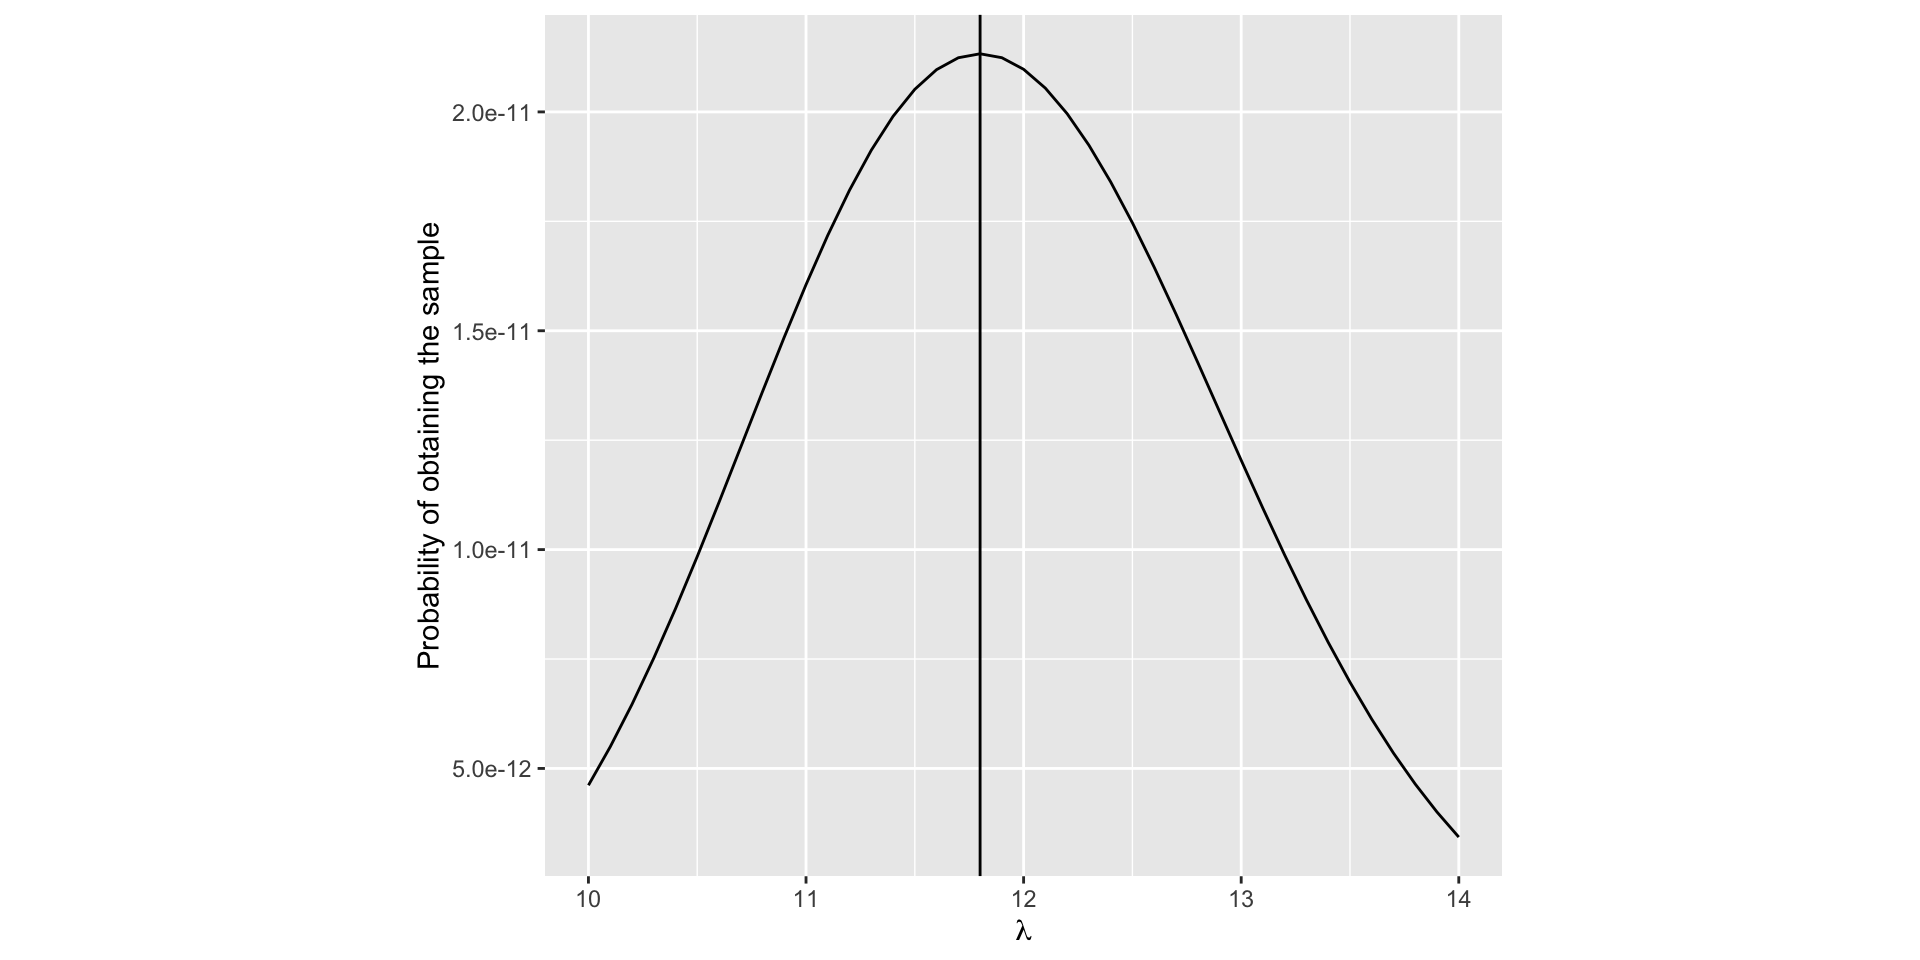
\includegraphics{figure/joint-1} 

}

\caption{Probability of the sample is maximum when $\lambda = 11.8$}\label{fig:joint}
\end{figure}

\begin{itemize}
\item
  When it is viewed as a function of \(\lambda\), it is called the \textbf{likelihood function of \(\lambda\) for the available data}
\item
  The likelihood for the data is maximum when \(\lambda = 11.8.\)
\item
  Since these data have already occurred, it is very likely that the data have arisen from a Poisson distribution with \(\lambda =11.8\).
\item
  This estimate for \(\lambda\) is called the \textbf{maximum likelihood estimate}
\item
  In order to define maximum-likelihood estimators, we shall first define the likelihood function.
\end{itemize}

\textbf{Definition: Likelihood function}

Let \(x_1,x_2, \dots, x_n\) be a set of observations of random variables \(X_1, X_2, \dots, X_n\) with the joint density of \(n\) random variables, say \(f_{X_1, X_2, \dots, X_n}(x_1,x_2, \dots, x_n;\; \theta)\). This joint density function, which is considered to be a function of \(\theta\) is called the \textbf{likelihood function of \(\theta\) for the set of observations (sample) \(x_1,x_2, \dots, x_n.\)}

In particular, if \(x_1,x_2, \dots, x_n\) is a random sample from the density \(f(x; \theta)\), then the likelihood function is \(f(x_1; \theta)f(x_2; \theta) \dots f(x_n; \theta).\)

\emph{Notation}

We use the notation \(L(\theta;\;x_1,x_2, \dots, x_n)\) for the likelihood function, in order to remind ourselves to think of the likelihood function as a function of \(\theta.\)

\begin{itemize}
\tightlist
\item
  Likelihood function is seen as a function of \(\theta\) rather than \(x\)
\item
  Likelihood can be viewed as the degree of plausibility.
\item
  An estimate of \(\theta\) may be obtained by choosing the most plausible value, i.e., where the likelihood function is maximized.
\end{itemize}

\textbf{Definition: Maximum Likelihood Estimator}

Let \(L(\theta)=L(\theta;\;x_1,x_2, \dots, x_n)\) be the likelihood function of \(\theta\) for the sample \(x_1,x_2, \dots, x_n.\) Suppose \(L(\theta)\) has its maximum when \(\theta = \hat{\theta}.\)

Then \(\hat{\theta}\) is called the \textbf{Maximum likelihood estimate of} \(\theta\).

The corresponding estimator is called the \textbf{Maximum likelihood estimator of} \(\theta\).

\begin{itemize}
\tightlist
\item
  Many likelihood functions satisfy regularity conditions; so the maximum likelihood estimator is the solution of the equation \[\frac{dL(\theta)}{d\theta} = 0\]
\end{itemize}

\textbf{Log-likelihood function}

Let \[l(\theta) = ln[L(\theta)].\]

Then, \(l(\theta)\) is called the \textbf{log-likelihood function}.

\begin{itemize}
\tightlist
\item
  Both \(L(\theta)\) and \(l(\theta)\) have their maxima at the same value of \(\theta\).
\item
  It is sometimes easier tot find the maximum of the logarithm of the likelihood and thereby simplify the calculations in finding the maximum likelihood estimate.
\end{itemize}

\textbf{Invariance Property of MLE's}

If \(\hat{\theta}\) is the MLE of \(\theta\), then for any function \(\tau(\theta),\) the MLE of \(\tau(\theta)\) is \(\tau(\hat{\theta}).\)

\newpage

\hypertarget{desirable-properties-of-point-estimators}{%
\subsection{Desirable properties of point estimators}\label{desirable-properties-of-point-estimators}}

\begin{itemize}
\item
  We discussed several methods of obtaining point estimators.
\item
  It is possible that different methods of finding estimators will lead to same estimator or different estimators.
\item
  In this section we discuss certain properties, which an estimator may or may not posses, that will guide us in deciding whether one estimator is better than another.
\end{itemize}

\hypertarget{unbiasedness}{%
\subsubsection{Unbiasedness}\label{unbiasedness}}

\textbf{Definition: Unbiased estimator}

An estimator \(\hat{\theta}\) \((=t(X_1, X_2, \dots, X_n))\) is defined to be an \textbf{unbiased estimator} of \(\theta\) if and only if
\[E(\hat{\theta}) = \theta\]

\begin{itemize}
\item
  The difference \(E(\hat{\theta}) -\theta\) is called as the bias of \(\hat{\theta}\) and denoted by
  \[Bias(\hat{\theta}) = E(\hat{\theta}) - \theta \]
\item
  An estimator whose bias is equal to 0 is called \textbf{unbiased}.
\end{itemize}

\hypertarget{consistency}{%
\subsection{Consistency}\label{consistency}}

\textbf{Mean-Squared Error}

\begin{itemize}
\tightlist
\item
  The \emph{mean-squared error} is a measure of goodness or closeness of an estimator to the target.
\end{itemize}

\textbf{Definition: Mean-squared Error (MSE)}

The \textbf{mean-squared error} of an estimator \(\hat{\theta}\) of \(\theta\) is defined as
\[MSE(\hat{\theta})= E\left[(\hat{\theta} - \theta)^2 \right]\]

\begin{itemize}
\item
  The MSE measures the average squared difference between \(\hat{\theta}\) and \(\theta\).
\item
  The MSE is a function of \(\theta\) and has the interpretation
\end{itemize}

\[MSE(\hat{\theta})= Var(\hat{\theta})+ \left[Bias(\hat{\theta}) \right]^2\]

\begin{itemize}
\item
  Therefore the MSE incorporates two components, one measuring the variability of the estimator (\emph{precision}) and the other measuring its bias (\emph{accuracy}).
\item
  Small value of MSE implies small combined variance and bias.
\item
  If \(\hat{\theta}\) is unbiased, then
  \[MSE(\hat{\theta})= Var(\hat{\theta})\]
\item
  The positive square root of MSE is known as the \emph{root mean squared error}
  \[RMSE(\hat{\theta})= \sqrt{MSE(\hat{\theta})}\]
\end{itemize}

\textbf{Consistency}

\begin{itemize}
\tightlist
\item
  Estimator \(\hat{\theta}\) is said to be consistent for \(\theta\) if \(MSE(\hat{\theta})\) approaches zero as the sample size \(n\) approaches \(\infty\).
\end{itemize}

\[lim_{n\rightarrow \infty}E\left[(\hat{\theta} - \theta)^2 \right]=0\]

\begin{itemize}
\tightlist
\item
  Mean-squared error consistency implies that the bias and the variance both approach to zero as \(n\) approaches \(\infty.\)
\end{itemize}

\newpage

\hypertarget{interval-estimation}{%
\section{Interval Estimation}\label{interval-estimation}}

\begin{itemize}
\item
  Under point estimation of a parameter \(\theta\), the inference is a guess of a \textbf{single value} as the value of \(\theta\).
\item
  Instead of making the inference of estimating the true value of the parameter to be a point, under interval estimation we make the inference of estimating that the true value of the parameter is contained in \textbf{some interval.}
\end{itemize}

\hypertarget{what-is-gained-by-using-an-interval-estimator}{%
\subsection{What is gained by using an Interval Estimator?}\label{what-is-gained-by-using-an-interval-estimator}}

\textbf{Example}

\begin{itemize}
\item
  For a sample \(X_1, X_2, X_3, X_4\) from a \(N(\mu, 1),\) an interval estimator of \(\mu\) is \([\bar{X}-1, \bar{X}+1].\)
\item
  This means that we will assert that \(\mu\) is in this interval.
\item
  In the previous section (Point estimation) we estimated \(\mu\) with \(\bar{X}.\)
\item
  But now we have the less precise estimator \([\bar{X}-1, \bar{X}+1]\).
\item
  Under interval estimation, by giving up some precision in our estimate (or assertion about \(\mu\)), we try to gain some confidence , or assurance that our assertion is correct.
\end{itemize}

\textbf{Explanation}

\begin{itemize}
\item
  When we estimate \(\mu\) by \(\bar{X},\) the probability that the estimator exactly equaled the value of the parameter being estimated is zero (Why? the probability that a continuous random variable equals any value is 0), \emph{i.e.} \(P(\bar{X}=\mu) = 0.\)
\item
  However, with an interval estimator, we have a positive probability of being correct.
\item
  The probability that \(\mu\) is covered by the interval \([\bar{X}-1, \bar{X}+1]\) can be calculated as
  \[P(\mu \in [\bar{X}-1, \bar{X}+1])= P(\bar{X}-1 \leq \mu\leq \bar{X}+1)\]
  \[ = P(-1 \leq \bar{X} - \mu\leq 1)\]
  \[ = P(- 2\leq \frac{\bar{X} - \mu}{\sqrt{1/4}}\leq 2)\]
  \[ = P(- 2\leq Z\leq 2)\;\;\; \left(\frac{\bar{X} - \mu}{\sqrt{1/4}} \text{ is standard normal }\right)\]
  \[=0.9544.\]
\item
  Therefore now we have over 95\% chance of covering the unknown parameter with the interval estimator.
\item
  By moving for a point to an interval we have scarified some precision in our estimate. But it has resulted in increased confidence that our assertion is correct.
\item
  The purpose of using an interval estimator rather than a point estimator is to have some guarantee of capturing the parameter of interest.
\end{itemize}

\hypertarget{definition-of-confidence-interval}{%
\subsection{Definition of confidence interval}\label{definition-of-confidence-interval}}

\textbf{Definition}

Let \(X_1, X_2, \dots, X_n\) be a random sample from a distribution with parameter \(\theta.\) Let \(T_1 = g(X_1, X_2, \dots, X_n),\) and \(T_2 = h(X_1, X_2, \dots, X_n)\) be two statistics satisfying \(T_1 \leq T_2\) for which \(P(T_1 < \theta < T_2)= \gamma,\) where \(\gamma\) does not depend on \(\theta\). Then, the random interval \((T_1, T_2)\) is called a \(100\gamma\) \textbf{percent confidence interval for} \(\theta\); \(\gamma\) is called the confidence coefficient; and \(T_1\) \(T_2\) are called the lower and upper confidence limits, respectively, for \(\theta.\)

Suppose that \(x_1, x_2, \dots, x_n\) is a realization of \(X_1, X_2, \dots, X_n\) and let \(t_1 = g(x_1, x_2, \dots, x_n),\) and \(t_2 = h(x_1, x_2, \dots, x_n)\). Then the \emph{numerical} interval \((t_1, t_2)\) is also called a \(100\gamma\) \textbf{percent confidence interval for} \(\theta\).

\hypertarget{interpretation-of-confidence-intervals}{%
\subsection{Interpretation of confidence intervals}\label{interpretation-of-confidence-intervals}}

\begin{itemize}
\item
  Consider the probability statement \(P(\bar{X}-1.18 \leq \mu\leq \bar{X}+1.18) =0.95.\)
\item
  The above probability statement implies that the random interval \((\bar{X}-1.18, \bar{X}+1.18)\) includes the unknown true mean \(\mu\) with probability 0.95.
\end{itemize}

\newpage

\hypertarget{methods-of-finding-interval-estimators}{%
\subsection{Methods of finding interval estimators}\label{methods-of-finding-interval-estimators}}

\hypertarget{pivotal-quantity-method}{%
\subsubsection{Pivotal Quantity Method}\label{pivotal-quantity-method}}

\textbf{Definition: Pivotal Quantity}

Let \(X_1, X_2,\dots, X_n\) be a random sample from the density \(f(.;\theta).\) Let \(Q=q(X_1, X_2,\dots, X_n; \theta)\); that is, let \(Q\) be a function of \(X_1, X_2,\dots, X_n\) and \(\theta\). If \(Q\) has a distribution that does not depend on \(\theta\), then \(Q\) is defined to be a \emph{pivotal quantity}

\textbf{Pivotal Quantity method}

If \(Q=q(X_1, X_2,\dots, X_n; \theta)\) is a pivotal quantity and has a probability density function, then for any fixed \(0<\gamma<1\) there will exist \(q_1\) and \(q_2\) depending on \(\gamma\) such that \(P[q_1<Q<q_2]=\gamma.\) Now, if for each possible sample value \((x_1, x_2, \dots, x_n),\) \(q_1< q(x_1, x_2,\dots, x_n; \theta)< q_2\) if and only if \(t_1(x_1, x_2,\dots, x_n)<\tau(\theta)<t_2(x_1, x_2,\dots, x_n)\) for functions \(t_1\) and \(t_2\) (not depending on \(\theta\)), then \((T_1, T_2)\) is a \(100\gamma\) percent confidence interval for \(\tau(\theta),\) where \(T_1=t_1(X_1, X_2,\dots, X_n)\) and \(T_2=t_2(X_1, X_2,\dots, X_n)\).

\hypertarget{methods-of-evaluating-interval-estimators}{%
\subsection{Methods of evaluating interval estimators}\label{methods-of-evaluating-interval-estimators}}

\begin{itemize}
\tightlist
\item
  Coverage probability
\item
  Size (expected length)
  \newpage
  \pagenumbering{arabic}
\end{itemize}

\hypertarget{tutorial-1}{%
\section*{Tutorial}\label{tutorial-1}}
\addcontentsline{toc}{section}{Tutorial}

\begin{enumerate}
\def\labelenumi{\arabic{enumi}.}
\item
  Let \(X_1, X_2, \dots, X_n \sim iid\;\; N(\mu, \sigma^2),\) both \(\mu\) and \(\sigma^2\) unknown. Derive a method of moment estimators for \(\mu\) and \(\sigma\).
\item
  Let \(X_1, X_2, \dots, X_n \sim iid\;\; Bin(n,\theta),\) both \(n\) and \(\theta\) unknown. Derive a method of moment estimators for \(n\) and \(\theta\).
\item
  Let \(X_1, X_2, \dots, X_n \sim iid\;\; Unif(\theta_1,\theta_2),\) where \(\theta_1<\theta_2\), both unknown. Derive a method of moment estimators for \(\theta_1\) and \(\theta_2\).
\item
  Let \(X_1, X_2, \dots, X_n \sim Poisson(\lambda).\) Derive a method of moment estimators for \(\lambda\).
\item
  Let \(X_1, X_2, \dots, X_n \sim iid\;\; Gamma(\alpha,\beta),\) both \(\alpha\) and \(\beta\) unknown. Derive a method of moment estimators for \(\alpha\) and \(\beta\).
\end{enumerate}

The survival time (in weeks) of 20 randomly selected male mouse exposed to 240 units of certain type of radiation are given below.

\(152, 115, 109, 94, 88, 137, 152, 77, 160, 165, 125, 40, 128, 123, 136, 101, 62, 153, 83, 69\)

It is believed that the survival times have a gamma distribution. Estimate the corresponding parameters.

\begin{enumerate}
\def\labelenumi{\arabic{enumi}.}
\setcounter{enumi}{5}
\tightlist
\item
  Let \(x_1, x_2, \dots, x_n\) be \(n\) random measurements of random variable \(X\) with the density function
  \[f_X(x;\lambda)= \lambda x^{\lambda-1},\;\; 0<x<1, \;\; \lambda>0\]
  Derive a method of moment estimator for \(\lambda\).
\end{enumerate}

\begin{enumerate}
\def\labelenumi{\arabic{enumi}.}
\setcounter{enumi}{6}
\item
  Let \(x_1, x_2, \dots, x_n\) be a random sample of size \(n\) from a Poisson distribution with parameter \(\lambda\). Derive the maximum likelihood estimator of \(\lambda\).
\item
  Let \(x_1, x_2, \dots, x_n\) be a random sample of size \(n\) from a normal distribution with mean \(\mu\) and variance \(\sigma^2\). Derive the maximum likelihood estimators of \(\mu\) and \(\sigma^2\).
\end{enumerate}

\begin{enumerate}
\def\labelenumi{\arabic{enumi}.}
\setcounter{enumi}{8}
\tightlist
\item
  Let \(X_1, X_2, \dots, X_n \sim iid \; Poisson (\lambda)\). Find the MLE of \(P(X\leq 1)\)
\end{enumerate}

\begin{enumerate}
\def\labelenumi{\arabic{enumi}.}
\setcounter{enumi}{9}
\tightlist
\item
  Let \(X_1, X_2, \dots, X_n \sim iid \; N (\mu, \sigma^2)\). Find the MLE of \(\mu/\sigma\).
\end{enumerate}

\begin{enumerate}
\def\labelenumi{\arabic{enumi}.}
\setcounter{enumi}{10}
\tightlist
\item
  Let \(X_1, X_2, \dots, X_n\) be a random sample from an exponential distribution with the density function
  \[f_X(x;\lambda)= \lambda e^{-\lambda x},\;\; x>0\]. Is the maximum likelihood estimators of \(\lambda\) unbiased?
\end{enumerate}

\begin{enumerate}
\def\labelenumi{\arabic{enumi}.}
\setcounter{enumi}{11}
\tightlist
\item
  Let \(X_1, X_2, \dots, X_n\) be a random sample of size \(n\) from a distribution with mean \(\mu\) and variance \(\sigma^2\). Show that \(\bar{X}\) and \(S^2 = \frac{\sum_{i=1}^n(X_i-\bar{X})^2}{n-1}\) are unbiased estimators of \(\mu\) and \(\sigma^2\), respectively.
\end{enumerate}

\begin{enumerate}
\def\labelenumi{\arabic{enumi}.}
\setcounter{enumi}{12}
\tightlist
\item
  Let \(x_1, x_2, \dots, x_n\) be a random sample of size \(n\) from a normal distribution with mean \(\mu\) and variance \(\sigma^2\). Consider the maximum likelihood estimators of \(\sigma^2\). Show the estimator \(\hat{\sigma^2} = \frac{\sum_{i=1}^n(X_i-\bar{X})^2}{n}\) is biased for \(\sigma^2\), but it has a smaller MSE than \(S^2 = \frac{\sum_{i=1}^n(X_i-\bar{X})^2}{n-1}\).
\end{enumerate}

\begin{enumerate}
\def\labelenumi{\arabic{enumi}.}
\setcounter{enumi}{13}
\tightlist
\item
  Let \(X_1, X_2, \dots, X_n\) be a random sample from some distribution and \(E(X) = \mu\). Show that \(\bar{X}\) is a better estimator than \(X_1\) and \(\frac{X_1+X_2}{2}\) for \(\mu\) in terms of MSE.
\end{enumerate}

\begin{enumerate}
\def\labelenumi{\arabic{enumi}.}
\setcounter{enumi}{14}
\tightlist
\item
  Let \(X_1, X_2, \dots, X_n\) be a random sample from a \(N(\mu, \sigma^2).\) Let \(\bar{X}= \frac{\sum_{i=1}^nX_i}{n}\) and \(T=\frac{\sum_{i=1}^n(X_i-\bar{X})^2}{n}\). Show that \(\bar{X}\) is consistent for \(\mu\) and \(T\) is consistent for \(\sigma^2.\)
\end{enumerate}

\begin{enumerate}
\def\labelenumi{\arabic{enumi}.}
\setcounter{enumi}{15}
\tightlist
\item
  Let \(X_1, X_2, \dots, X_n\) be a random sample from a \(N(\mu,9).\) Find a 95\% confidence interval for \(\mu\).
\end{enumerate}

\begin{enumerate}
\def\labelenumi{\arabic{enumi}.}
\setcounter{enumi}{16}
\tightlist
\item
  Let \(X_1, X_2, \dots, X_n\) be a random sample from a \(N(\mu,\sigma^2),\) both \(\mu\) and \(\sigma\) are unknown. Construct a \(100(1-\alpha)\%\) \((0<\alpha<1)\) confidence interval for \(\mu\).
\end{enumerate}

\begin{enumerate}
\def\labelenumi{\arabic{enumi}.}
\setcounter{enumi}{17}
\tightlist
\item
  Let \(X_1, X_2, \dots, X_n\) be a random sample from a \(N(\mu,\sigma^2),.\) Construct a \(100(1-\alpha)\%\) \((0<\alpha<1)\) confidence interval for \(\sigma^2\).
\end{enumerate}

\hypertarget{hypothesis-testing}{%
\chapter{Hypothesis Testing}\label{hypothesis-testing}}

\hypertarget{null-and-alternative-hypotheses}{%
\section{Null and alternative hypotheses}\label{null-and-alternative-hypotheses}}

\hypertarget{errors-in-testing-hypotheses-type-i-and-type-ii-error}{%
\section{Errors in testing hypotheses-type I and type II error}\label{errors-in-testing-hypotheses-type-i-and-type-ii-error}}

\hypertarget{significance-level-size-power-of-a-test}{%
\section{Significance level, size, power of a test}\label{significance-level-size-power-of-a-test}}

\hypertarget{formulation-of-hypotheses}{%
\section{Formulation of hypotheses}\label{formulation-of-hypotheses}}

\hypertarget{methods-of-testing-hypotheses}{%
\section{Methods of testing hypotheses}\label{methods-of-testing-hypotheses}}

\hypertarget{design-of-experiments}{%
\chapter{Design of Experiments}\label{design-of-experiments}}

\hypertarget{ntroduction-to-experimental-design}{%
\section{ntroduction to experimental design}\label{ntroduction-to-experimental-design}}

\hypertarget{basic-principles-of-experimental-design}{%
\section{Basic principles of experimental design}\label{basic-principles-of-experimental-design}}

\hypertarget{completely-randomized-design}{%
\section{Completely randomized design}\label{completely-randomized-design}}

Casella, G., \& Berger, R. L. (2002). Statistical inference (Vol. 2, pp.~337-472).Pacific Grove, CA: Duxbury

Mood, A.M., Graybill, F.A. and Boes, D.C. (2007): Introduction to the Theory of Statistics, 3rd Edn. (Reprint). Tata McGraw-Hill Pub. Co.~Ltd.

\bibliography{book.bib,packages.bib}

\end{document}
